%\documentclass[]{thesis}  % draft mode (default)
%\documentclass[review]{thesis}  % review mode (show contents & reference only)
\documentclass[watermark,final]{thesis}  % final mode (version for library)

%-------------------------------------------------------------------------------
% Package Loading
%-------------------------------------------------------------------------------

\usepackage{cite}
\usepackage{wallpaper}

\usepackage{multirow}     % for multi-row table
\usepackage{booktabs}     % table style used in books
\usepackage{chngcntr}     % make figure indexing sequential
\usepackage{rotating}     % make figure rotating
\usepackage{amssymb}      % math symbol
\usepackage{algpseudocode}
%-------------------------------------------------------------------------------
% Configuration
%-------------------------------------------------------------------------------

% 填寫題目, 作者, 指導教授, 學校, 系所, 日期等資訊
% Title
\title{Unseen defect image synthesis with compositional conditional diffusion model}
\titlezh{基於條件擴散模型的未見缺陷圖像合成 }

% Author
\author{Pin-Chuan Chen}
\authorzh{陳品銓}

% Advisor
\advisor{Ching-Wen Ma}
\advisorzh{馬清文}

% First co-advisor (Leave {} empty if you don't have a co-advisor)
\coadvisorA{}
\coadvisorAzh{}

% Second co-advisor (Leave {} empty if you don't have a second co-advisor)
\coadvisorB{}
\coadvisorBzh{}

% Field
\field{Artificial Intelligence}

% Institute
\institute{Institute of Computational  Intelligence}
\institutezh{智慧計算與科技研究所}

% College
\college{College of Artificial Intelligence}

% University
\university{National Yang Ming Chiao Tung University}
\universityzh{國立陽明交通大學}

% Location
\location{Taiwan, Republic of China}

% Date of final submission
\degreemonth{May}
\degreeyear{2024}
\degreeyearzh{中華民國 一一三年五月}

% Date of final submission
\nation{中華民國}
\yearmonth{一一三年五月}

% Watermark %At present(v.1 2021.Sep.29, v.2 2022.Feb.25), not water wark for NYCU yet.
% \watermark{figures/nycu_logo_1.png}

% 修改 thesis.cls 的預設字型
%-------------------------------------------------------------------------------
% Chinese Font Settings
%
%   These macros are used to change the default Chinese fonts (see below) used
% by thesis.cls. Please leave {} empty if you want to use the default settings
% and make sure that you have added '-shell-escape' option when using xetex to
% compile tex files, i.e. xetex compiling commands should run something like:
%
%     xelatex -synctex=1 -shell-escape -interaction=nonstopmode %.tex
%
% (default Chinese font settings)
%   Windows              Linux                        Mac OS X
% * 標楷體 (DFKai-SB)    AR PL 中楷 (AR PL UKai TW)   楷體-繁 (Kaiti TC Regular)
% @ 新細明體 (PMingLiU)  AR PL 明體 (AR PL UMing TW)  儷宋 Pro (LiSong Pro)
%
% * fontname --> 預設中文本文字型 (serif)
% @ fontname --> 預設中文明體字型 (sans-serif, 使用於封面頁)
%-------------------------------------------------------------------------------

% main (serif) Chinese font, leave {} empty to enable default font setting
\mainfontzh{}

% sans-serif Chinese font, leave {} empty to enable default font setting
\sansfontzh{}

%-------------------------------------------------------------------------------
% English Font Settings
%
%   These macros are used to change the default English fonts (see below) used
% by thesis.cls. Please leave {} empty if you want to use the default settings.
%
% (default English font settings)
% main font       --> Times New Roman (for all platforms)
% sans-serif font --> Arial           (for all platforms)
%-------------------------------------------------------------------------------

% main font for English, leave {} empty if you want to use default font setting
\mainfont{}

% sans-serif font for English, leave {} empty if you want to use default setting
\sansfont{}



\begin{document}

% Show repeated author names in bibliography when using IEEEtran.bst
% Comment out this line if you don't set IEEEtran in \bibliographystyle{}
\bstctlcite{IEEEexample:BSTcontrol}

% Generate cover, title, authorization, approval and copyright pages
\maketitle

% 題獻頁 (Only shown in the final mode of a PhD dissertation)
\begin{dedication}%

\textit{Dedicated to Cosmic Ray Lab $@$ NCTU}\\

{\Large 為了善用所辦的咖啡機, 工作前要喝一杯咖啡.}\\

\end{dedication}

%-------------------------------------------------------------------------------
% Abstract
%-------------------------------------------------------------------------------

% 中文摘要
\begin{abstractzh}

血管通路功能不全是透析患者常見且嚴重的併發症,尤其在透析患者比例全球最高的台灣,早期診斷和管理顯得尤為重要。傳統的診斷方法,如定期監測及固定血流量閾值的應用,難以找出潛在需要執行手術的病患。為解決此問題,本研究提出了一個具備不確定感知能力的樹狀機器學習框架,旨在改善血管通路功能不全的判斷方法。

該框架結合了Decision Trees、Random Forests及XGBoost等樹狀模型,並融入了先進的不確定性量化技術。通過多次擾動的方式模擬樣本的變化,實現了對不確定樣本的識別。本研究還引入了擴展混淆矩陣及創新的不確定性指標,從多角度對模型性能進行全面評估。從實驗與驗證結果表明,該框架相較於傳統方法(如KDOQI guidelines)具有更高的預測準確性和敏感性。將模棱兩可的樣本分類為不確定樣本的能力提升了臨床決策的可靠性,避免了過於自信的誤判並減少了不必要的干預。本研究在醫院的真實資料集中進行模擬,驗證所提出之方法的性能。

\vspace{5cm}

關鍵詞: 血管通路功能不全、樹模型、機器學習、不確定性量化

\end{abstractzh}

% 英文摘要
\begin{abstract}%

In typical machine learning tasks, the test dataset usually shares the same distribution as the training dataset. Similarly, in the domain of image generation, the generation models often produce data with the same distribution as the training dataset. We addressed this limitation by employing various methods to achieve unseen data generation using a simple example. When existing methods failed to accomplish this, we further decomposed unseen data generation into unseen compositional image generation. We guided the generation model using compositional class labels. Unlike traditional approaches that use a single class label to guide the generation process, our model uses multiple category labels, such as attribute categories and object categories, to control the generation process. Through training, the model learns features from different types of labels to achieve compositional zero-shot image generation.

Regarding zero-shot generation, large language models like GPT-4 and large-scale image generation models like DALL-E 2 also possess similar zero-shot generation capabilities. However, our research focuses on implementing zero-shot generation within specific domains and using smaller models. To demonstrate the potential and prerequisites of compositional zero-shot image generation as a task achievable with contemporary machine learning techniques, we designed a series of tasks ranging from simple to complex compositional zero-shot generation tasks. In the simpler tasks, our proposed method accurately generates new compositional samples. In the more complex tasks, the newly generated compositional samples from our model, when selected appropriately, also yield reasonable new samples.

\vspace{17cm}

Keyword: Image generation, Diffusion Model, Compositional zero-shot image generation, Compositional zero-shot learning 

\end{abstract}

%-------------------------------------------------------------------------------

% 目錄
%-------------------------------------------------------------------------------

% Generate 'Table of Contents', 'List of Figures', and 'List of Tables', and
% Set page numbering to 'arabic'
\maketocs

%-------------------------------------------------------------------------------
% Contents
%-------------------------------------------------------------------------------

% Set page numbering to 'arabic' (1, 2, 3, ...)
\mainmatter

% 內文, 請依照章節順序擺放
\chapter{Introduction}
\label{chapter:intro}


\section{Background}
Image generation is a process that involves utilizing computer algorithms and models to create new images. This intricate process typically incorporates mathematical and statistical methods, along with extensive training data, enabling computers to generate images with diverse visual features and structures. By leveraging existing data and models, the computational system can produce highly realistic images.

In practical applications, components can be categorized into "old components," which have ample normal and defective samples, and "new components," where defective samples may be insufficient or lacking. It is crucial to note that the types of defects for both new and old components are identical, as detailed in Table 1.1.
\renewcommand{\arraystretch}{1.5} % 调整行高
\setlength{\tabcolsep}{10pt} % 调整列间距

\begin{table}[h]
    \centering
    \begin{tabular}{lll} \hline  
         &  Normal& Defect\\ \hline  
         New component&  Numerous& Numerous\\ \hline  
         Old componet&Numerous&Several or None\\ \hline 
    \end{tabular}
    \caption{The types of defects for both new and old components}
    \label{tab:my_label}
\end{table}
Traditional models exhibit suboptimal performance in generating defects for new components. Consequently, our research focuses on designing a more effective model structure for generating defect features when only defective samples from old components are available.

The challenge lies in innovatively addressing the deficiency of defect samples for new components, thereby enhancing the model's ability to generate realistic and diverse defect features. Through this research, we aim to contribute to the advancement of image generation techniques, particularly in scenarios where limited or no defect data is available for new components.


\section{Motivation}
Taiwan's Printed Circuit Board (PCB) industry holds the leading position in global market share. For PCB manufacturers, the yield rate of circuit boards is crucial; a poor yield rate not only increases costs but also damages corporate reputation. Some manufacturers employ Artificial Intelligence (AI) to develop "Defect Detection" systems, significantly enhancing product quality and inspection efficiency. However, these systems perform poorly in identifying defect types in unseen components, necessitating the use of image generation technology.

Welding is a common technique in industrial manufacturing, involving the connection of electronic components. However, the welding process introduces challenges such as high temperatures, high pressures, and the potential for chemical reactions, making it susceptible to defects. These defects can disrupt the entire manufacturing process or result in subpar quality of the final product. Therefore, the development of imaging techniques capable of generating images of defects in new components becomes crucial.

In the current field of image generation, text-to-image techniques, such as OpenAI's Stable Diffusion\cite{Stable_Diffusion} method, are widely applied. However, in our experiments, the goal is not to generate generalized patterns but rather specific images related to industrial manufacturing. When providing descriptions of our industrial components to ChatGPT, converting them into prompts, and subsequently utilizing Stable Diffusion for image generation, we observed significant discrepancies and even errors in the generated images.

In addressing these challenges, the use of Conditional Diffusion Models(CDMs) demonstrates significant potential, particularly in handling complex variation processes. The distinctive feature of CDMs lies in their ability to generate images with specific features based on different conditions. They not only model common defect characteristics but also generate corresponding defect images based on the characteristics of different components.

The use of CDMs helps overcome the deficiency of defect samples for new components. By learning from existing data, these models can generate a broader range of defect scenarios based on class conditions, to enhance the accuracy of generating defect images. This, in turn, contributes to minimizing disruptions in the entire manufacturing process and preventing a decline in product quality.


\section{Goal}
The PCB dataset used in this study was provided by a collaborative industry partner of our laboratory, and was used previously for defect detection research. In the initial phase of this project, the dataset was used to investigate the generation of "zero-shot" images, and it will be employed as an augmented dataset for defect detection in the subsequent stages of this research.

As shown in Figure 1.1, we present the representation of component groups and defect types. It can be observed that the combination within the "Broke Group3" is not present in this dataset.
\begin{figure}[H]
    \centering
    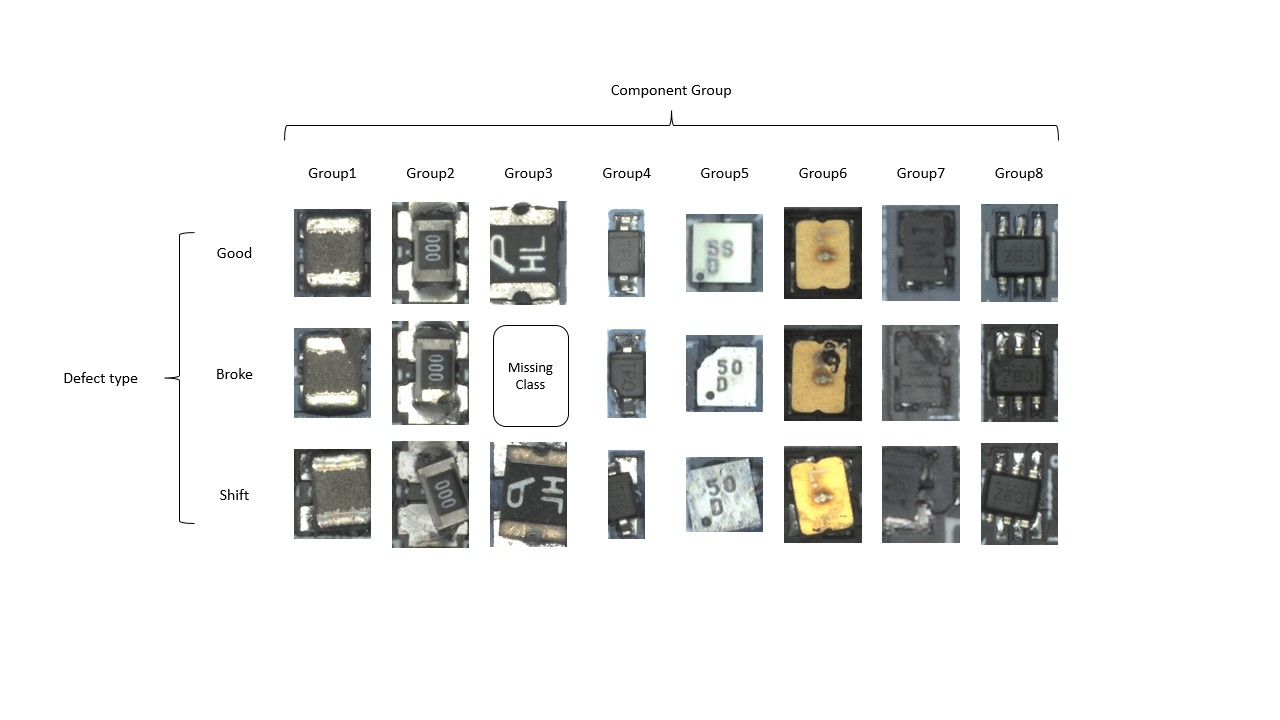
\includegraphics[width=1\linewidth]{Goal.jpg}
    \caption{The representation of component groups and defect types }
    \label{fig:enter-label}
\end{figure}

This study aims to employ an estimation method based on diffusion processes, utilizing a Compositional Class-to-image approach to generate defect images for new components (Broke Group3). The produced new components (Broke Group3) will be integrated into the defect component detection model to enhance the model's generalization ability to unseen images. Additionally, we implement Denoising Diffusion Implicit Models(DDIM)\cite{DDIM} sampling to expedite the generation process. The overarching goal is to provide direction and inspiration for future research in this domain.


\section{Contribution}
The contributions of this thesis are summarized in the following:
\begin{itemize}
    \item We propose a novel class-to-image generation method that reduces training time by eliminating the need for additional text pre-training models, such as CLIP\cite{CLIP}.
    \item Unlike traditional prompts requiring lengthy descriptions, our method does not rely on complex textual inputs yet is capable of producing accurate and exceptional images even in unseen contexts. This approach simplifies the generation process while ensuring both accuracy and diversity in the generated images.
    \item \textbf{Novelty in New Component Defect Generation Model}: Our study pioneers the use of the Compositional Conditional Diffusion method for generating defects in previously unseen new components. This groundbreaking approach represents a new contribution to the field, introducing a unique and innovative model for defect generation.
    \item \textbf{Practical Application Scenarios}: The potential real-world impact of our model, especially in the industrial welding domain, underscores its practical utility. This application-oriented contribution enhances the relevance and applicability of our research in addressing challenges within the welding industry.
\end{itemize}


\chapter{Related Works}
\label{chapter:doccls}

\section{KDOQI Guidelines}

The 2006 update to the KDOQI guidelines~\cite{KDOQI} offers a comprehensive framework for managing vascular access in hemodialysis patients, addressing aspects from patient evaluation to long-term access maintenance. This update, based on studies conducted between 1997 and 2005, aims to reduce vascular access-related morbidity and improve long-term functionality. The guidelines include evidence-based recommendations for creating and maintaining arteriovenous fistulas (AVFs) and grafts (AVGs), highlighting specific thresholds for vascular flow rates: AVFs with flow rates below 500 mL/min and AVGs below 600 mL/min should be further evaluated for potential stenosis or dysfunction.

However, relying solely on these flow rate thresholds may not be sufficient for optimal decision-making regarding interventions. Recent studies have explored the integration of artificial intelligence (AI) and machine learning techniques to enhance surgical decision-making processes. For instance, AI-enabled clinical decision~\cite{Balch_2024} support systems have shown promise in improving surgical outcomes by analyzing complex datasets to predict patient-specific risks and recommend tailored interventions.These advancements suggest that incorporating AI into clinical practice could augment traditional guidelines, leading to more precise and individualized patient care.

In summary, while the KDOQI guidelines provide a solid foundation for vascular access management in hemodialysis patients, integrating AI and machine learning approaches holds the potential to further refine surgical decision-making, thereby enhancing patient outcomes.

\section{Physical Examination}

Regular vascular access blood flow (Qa) surveillance~\cite{Wu}, combined with routine clinical monitoring and physical examination, has proven effective in predicting vascular access stenosis in chronic hemodialysis patients. By analyzing data from 397 patients with arteriovenous fistulas (AVF) and arteriovenous grafts (AVG), this approach identifies optimal Qa thresholds for detecting stenosis. Absolute thresholds of <500 mL/min for AVF and <600 mL/min for AVG demonstrate high predictive performance, achieving accuracy rates of 91.54\% and 72.15\%, respectively. Additionally, a stricter threshold of <400 mL/min for AVF is proposed as an alternative criterion for enhanced specificity. These absolute thresholds outperform relative thresholds, which incorporate both absolute Qa levels and a 25\% decline from previous measurements, underscoring the reliability of absolute benchmarks in clinical decision-making.

Integrating these thresholds with physical examinations addresses the inherent limitations of clinical monitoring alone. While AVF patients benefit significantly from this combined approach, challenges remain for AVG patients due to structural differences in grafts, necessitating supplementary diagnostic tools such as duplex ultrasound. This framework not only improves early stenosis detection but also highlights the value of multidisciplinary collaboration in vascular access management. Furthermore, it establishes a foundation for adopting advanced techniques, such as machine learning models, to enhance prediction accuracy and inform timely interventions.
\newpage
\section{Tree-based Approaches}

Tree-based machine learning models, such as Decision Trees, Random Forests, and XGBoost, represent foundational and advanced techniques widely used in structured data analysis. These methods have evolved to balance interpretability, computational efficiency, and predictive accuracy, addressing key challenges in traditional machine learning approaches.

Decision Trees~\cite{decision_tree} form the basis of tree-based methods, utilizing recursive splitting to categorize or predict outcomes. Despite their simplicity and high interpretability, Decision Trees are prone to overfitting, especially in complex, high-dimensional datasets. To address this limitation, ensemble techniques like Random Forests~\cite{random_forest} and XGBoost~\cite{XGBoost} have emerged. Random Forests employ bagging (bootstrap aggregating), which involves training multiple decision trees on random subsets of data and aggregating their outputs. This method significantly reduces variance and enhances model stability, particularly in noisy or imbalanced datasets~\cite{comprehensive_tree_based_model}.

In contrast, XGBoost exemplifies the boosting paradigm, where weak learners are iteratively combined to minimize errors from previous iterations~\cite{Comparative_XGBoost}. XGBoost introduces advanced features like sparsity-aware algorithms and regularized objectives, making it highly efficient and scalable for large datasets. These innovations have positioned XGBoost as a dominant method in machine learning competitions and real-world applications, from clinical diagnostics to financial modeling~\cite{Yan_2020}. Recent comparative studies also highlight advancements in gradient boosting frameworks, such as LightGBM~\cite{LightGBM} and CatBoost~\cite{CatBoost}. While LightGBM excels in training speed through selective sampling techniques, CatBoost addresses prediction shifts caused by categorical feature encoding, further enhancing generalization performance. Together, these methods provide a comprehensive suite for structured data analysis, offering adaptability across diverse domains.

Tree-based models, such as XGBoost and Random Forests, often outperform neural networks on tabular data due to the unique characteristics of these datasets and the strengths of tree-based approaches. Tabular data typically consists of a mix of numerical and categorical features, irregular patterns, and skewed or heavy-tailed distributions, which tree-based models handle efficiently by learning piecewise constant functions. This allows them to capture irregular patterns, ignore irrelevant features, and adapt to data heterogeneity without extensive preprocessing or feature engineering. In contrast, neural networks struggle with these properties, requiring significant regularization and feature transformation to achieve comparable results.

Research supports these observations. Grinsztajn et al. (2022)~\cite{tree_based_model} demonstrate that tree-based models excel on medium-sized datasets (~10,000 samples), where neural networks often fail to generalize due to their reliance on smooth functions and their sensitivity to uninformative features. McElfresh and Khandagale (2023)~\cite{Outperform_Boosted_Trees} further highlight that Gradient Boosted Decision Trees (GBDTs) outperform neural networks on average, particularly in handling data irregularities and dataset-specific properties. Additionally, Ye et al. (2024)~\cite{Closer_Look} find that while deep learning has improved, tree-based models remain competitive, especially in scenarios with limited data or computational resources. These advantages, combined with their computational efficiency and minimal hyperparameter tuning requirements, make tree-based models a robust and practical choice for structured datasets, where neural networks' strengths in image and text data do not translate effectively.



\section{Ensemble Learning}

Ensemble learning has become a cornerstone in machine learning for enhancing model robustness and improving predictive accuracy by combining multiple base classifiers~\cite{9893798}. Two primary ensemble strategies, bagging and boosting, form the foundation of many successful machine learning models. Bagging methods, such as Random Forest, focus on reducing variance by training multiple classifiers independently and aggregating their outputs. This approach ensures stability and robust performance, particularly in datasets with noise or complex distributions.

In this study, we leverage the strengths of these ensemble methods by employing a soft voting classifier that combines Decision Trees, Random Forests, and XGBoost~\cite{Kim2018AutomatedML, Interpretable_tree_ensemble}. The soft voting approach integrates predictions probabilistically, assigning weights based on the confidence levels of individual models. This method captures both the diversity and the complementary strengths of the base classifiers, ensuring a more balanced and accurate prediction framework.

The decision to use a soft voting ensemble stems from its proven ability to manage structured data effectively. Unlike neural networks, which may struggle with limited structured datasets and interpretability, tree-based ensembles offer clear advantages in handling imbalanced data, feature interactions, and hierarchical relationships inherent in clinical and structured datasets.

\section{Indeterminacy Handling and Interpretability}

In this study, tree-based models were employed to address challenges in structured data classification by integrating Indeterminacy quantification and enhancing model interpretability. While the methods used are specific to tree-based models, the approach is inspired by concepts and techniques explored in other machine learning and deep learning research~\cite{Uncertainty_Quantification}.

Indeterminacy quantification is a critical aspect of this study, as it enables the model to effectively manage ambiguous cases and provide more reliable predictions. Insights from Indeterminacy modeling~\cite{Uncertainty_Quantification_2}  provide a foundational framework, offering methodologies to quantify both aleatoric and epistemic indeterminacies and evaluate their impact on predictive accuracy. These concepts guided the implementation of metrics and approaches tailored for tree-based models to improve their reliability and adaptability in structured data classification.

Another key influence is the use of Indeterminacy-based rejection techniques~\cite{electronics11030396}, which demonstrate the utility of quantifying prediction Indeterminacy to enhance model selection and enable the integration of diverse classifiers. Inspired by these strategies, this study incorporates mechanisms to reallocate highly indeterminate predictions to an "indeterminate" category, ensuring more cautious decision-making. This approach is particularly valuable in clinical applications where incorrect classifications could lead to significant consequences.

The focus on interpretability in this study also draws from methods that emphasize local perturbations to approximate complex model behavior~\cite{perturbations}, providing interpretable explanations for individual predictions. These techniques influenced the design of Indeterminacy-aware explanations for tree-based models, facilitating a deeper understanding of decision boundaries and feature contributions for each prediction.

Lastly, the study integrates principles inspired by methods that estimate Indeterminacy using randomness in model computations~\cite{pmlr-v48-gal16}. Although initially designed for neural networks, these concepts informed the multipass perturbation approach employed here, where noise is introduced into input features to analyze prediction variability. This method enables the approximation of Indeterminacy in ensemble tree-based models, extending the applicability of these ideas to structured data classification.

This integrated framework leverages existing advancements in Indeterminacy quantification and interpretability to adapt them for tree-based models, enabling robust and explainable predictions in complex real-world scenarios.
\chapter{Method}
\label{chapter:secorder}
This chapter describes the experimental methods and technical processes employed in this study and elaborates on how indeterminacy analysis can enhance the predictive capability and stability of the proposed models. The primary objective of this chapter is to propose an indeterminacy judgment method that predicts outcomes by introducing multiple instances of varying noise to the same sample, thereby quantifying indeterminacy and optimizing classification decisions accordingly.

The methodology presented in this chapter is structured into three main components. First, Section 3.1 outlines the data preprocessing techniques, the design of the machine learning models, and the training process used in this study. Second, Section 3.2 explains how multiple passes through perturbed samples are used to analyze sample indeterminacy and compute the probability means and variances of the predictions. Finally, Section 3.3 demonstrates how classification decisions are made based on the indeterminacy evaluation results, categorizing samples into "determinate" (True/False) or "indeterminate" (Indeterminate) classes.

In modern clinical applications, there is an increasing demand for diagnostic precision and robustness, particularly in the early detection of vascular access dysfunction. Traditional diagnostic approaches often rely on fixed blood flow thresholds, which can lead to misdiagnoses or missed diagnoses due to fluctuations in individual values. The primary goal of this study is to address this problem by introducing the concept of indeterminacy analysis, which adjusts classification decisions to ensure that the system provides more cautious diagnostic outcomes for ambiguous samples. The framework proposed in this chapter effectively addresses the limitations of traditional diagnostic methods, enabling the system to classify clear samples accurately while also offering indeterminacy evaluations for borderline cases, thereby enhancing its utility in clinical applications.

\begin{comment} 
Section ordering in \textit{thesis.cls} is:
\begin{itemize}
\item Chapter (shown in \textbf{Table of Contents})
\item Section (shown in \textbf{Table of Contents})
\item Subsection (shown in \textbf{Table of Contents})
\item Paragraph
\item Subparagraph
\end{itemize}
DONOT use \textbackslash subsubsection, it is not supported in \textit{thesis.cls}.
It is replaced by \textbackslash paragraph.
\end{comment}

\section{Model Architecture}
In this chapter, we introduce the proposed Indeterminacy Classification Model designed to classify samples, as illustrated in Figure 3.1.

\begin{figure}[H]
    \centering
    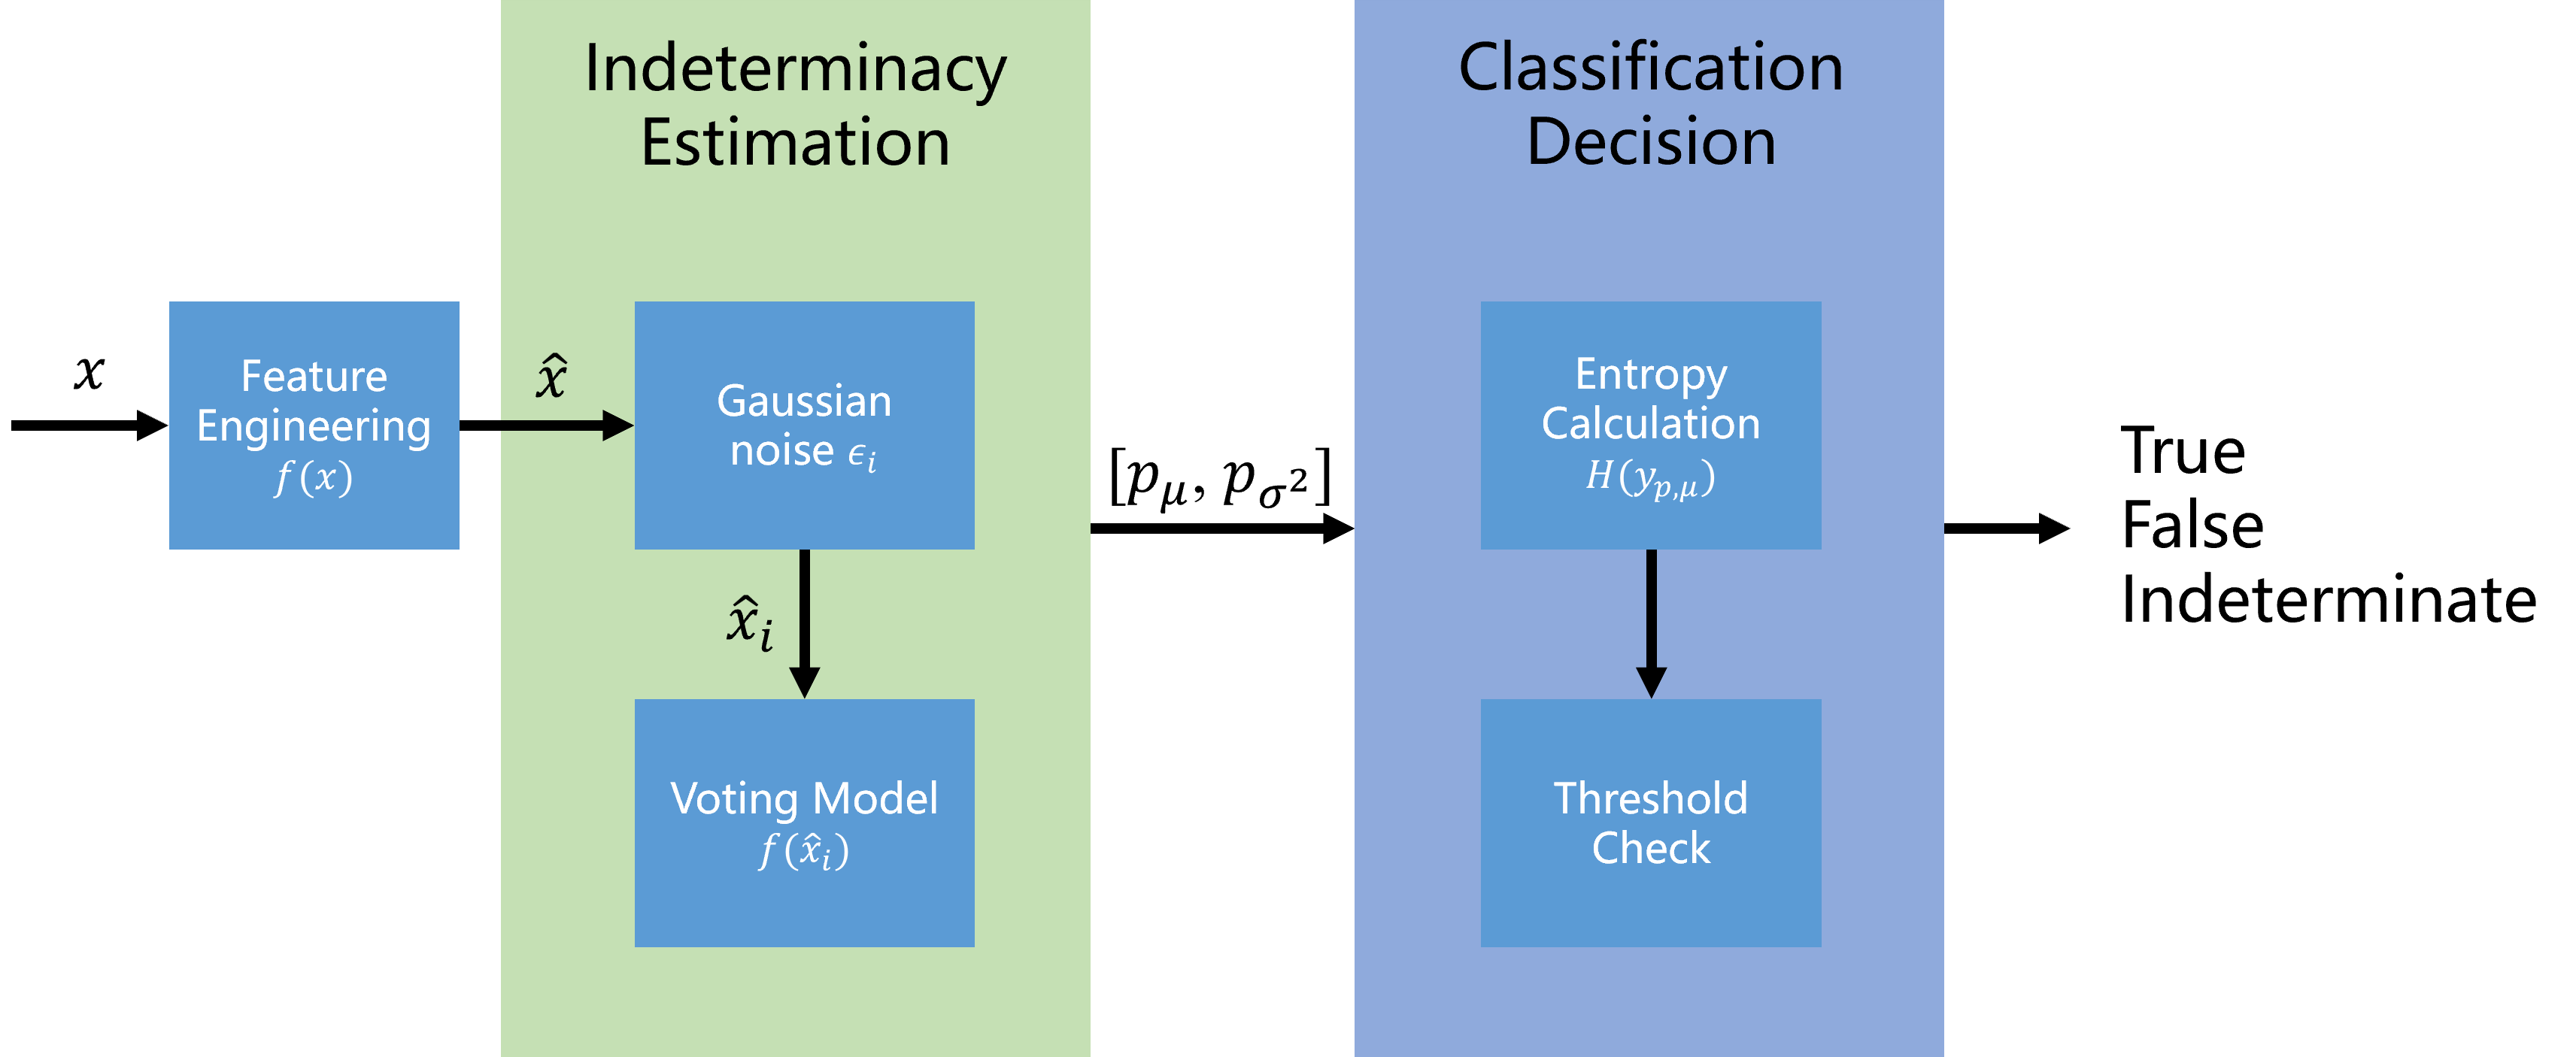
\includegraphics[width=1\linewidth]{figures/model_architecture.png}
    \caption{Indeterminacy Classification Model}
    \label{fig:enter-label}
\end{figure}

The structured dataset underwent preprocessing steps, which included removing redundant information, feature creation, and aligning the data. These steps ensure that the dataset is clean and suitable for training machine learning models. For a detailed explanation of the preprocessing steps, please refer to Chapter 4.2.

The models utilized in this study are tree-based machine learning classifiers, specifically:

\begin{itemize}
    \item \textbf{Decision Tree}: A fast and interpretable model; however, it is prone to overfitting when applied to high-dimensional data.
    \item \textbf{Random Forest}: An ensemble of decision trees that effectively reduces model variance and improves prediction stability.
    \item \textbf{XGBoost}: A gradient boosting framework renowned for its computational efficiency and strong classification performance, particularly in imbalanced datasets.
\end{itemize}

To leverage the strengths of these models, we implemented a weighted soft voting strategy, combining the prediction probabilities from each model. This approach allows the ensemble to capture diverse perspectives from the individual classifiers. Furthermore, to address the imbalance between positive and negative samples, we adjusted the \texttt{scale\_pos\_weight} parameter in XGBoost, ensuring that the model assigns appropriate importance to minority class samples. All models were trained and evaluated using K-fold cross-validation, which ensures robust and reliable performance.

After constructing the soft voting model, it was integrated into the Multipass Indeterminacy Estimation Method and the Indeterminate-Aware Data Classification process. These methods enhance the classification framework by quantifying and addressing indeterminacy, further improving the model's applicability in complex scenarios.

\section{Multipass Indeterminacy Estimation Method}% Algorithm
To quantify the indeterminacy of each sample, we propose the Multipass Indeterminacy Estimation Method. The key idea is to generate multiple perturbed versions of each sample by adding Gaussian noise $\epsilon=N(\mu,\sigma^2)$. Each perturbed version of the sample is then passed through the weighted soft voting classifier, which predicts the probabilities for True and False. The predicted probabilities for True and False across all perturbed versions are then aggregated to calculate their respective means ($p_{u}$) and variances ($p_{\sigma^2}$). This process is repeated for each sample individually.

The main steps of this method are:
\begin{enumerate}
  \item \textbf{Perturbed Sample Generation}: Adding Gaussian noise to the input features to simulate data indeterminacy, creating multiple perturbed versions of the sample.
  \item \textbf{Multi-Model Prediction}: Passing each perturbed version through the soft voting classifier, which integrates predictions from Decision Tree, Random Forest, and XGBoost to generate probabilities for $True$ and $False$.
  \item \textbf{Probability Mean and Variance Calculation}: Aggregating the predicted probabilities for True and False across all perturbed versions by calculating their respective means ($p_{u}$) and variances ($p_{\sigma^2}$).
\end{enumerate}

The use of multiple perturbed versions of a sample considers the fact that a patient’s current blood flow rate is not fixed but continuously fluctuating. By generating multiple perturbed inputs representing variations in blood flow rates for the same patient, the model can simulate real-world conditions. This approach enables the model to provide more confident and robust predictions under varying circumstances.

\begin{algorithm}[H]
\caption{Multipass Indeterminacy Estimation}
\label{alg:Training}
\begin{algorithmic}[1]
\Statex \textbf{Input:} 
\Statex \hspace{1em} \(\hat{x}\): Input sample, \(\mu\): Noise mean, \(\sigma^2\): Noise variance
\Statex \hspace{1em} \(W=[w_{1},w_{2},w_{3}]\): Weight of estimator, \(n\): Number of estimation times
\Statex \hspace{1em} \(Estimators\): \([Decision Tree, Random Forest, XGBoost]\)
\Statex \textbf{Output:} 
\Statex \hspace{1em} \(p_{\mu}\): Mean of probability, \(p_{\sigma^2}\): Variance of probability
\Statex \textbf{Initialize:}
\Statex \hspace{1em} $\hat{P}=[\hspace{1em}]$
\State \textbf{for} estimate \(i\) from \(1\) to \(n\) \textbf{do}
\State \hspace{1em} \(\epsilon_{i} \sim N(\mu,\sigma^2)\) 
\State \hspace{1em} \(\hat{x_{i}} \leftarrow \hat{x} + \epsilon_{i} \)
\State \hspace{1em} \(P_{y_{i}} = [\hspace{1em}]\)
\State \hspace{1em} \textbf{for} \(clf\) in \(Estimators\) \textbf{do}
\State \hspace{2em} \(v_{clf} = VotingClassifier(clf, voting = 'soft')\)
\State \hspace{2em} \(p_{y_{i}, clf} = v_{clf}.PredictProb(\hat{x_{i}})\) \(\# p=[p_{T},p_{F}]\)
\State \hspace{2em} Append \(p_{y_{i}, clf}\) to \(P_{y_{i}}\)
\State \hspace{1em} \textbf{end}
\State \hspace{1em} \(\hat{p_{i}}=average(P_{y_{i}}, W)\)
\State \hspace{1em} Append \(P_{y_{i}}\) to \(\hat{P}\)
\State \textbf{end}
\State \(p_{\mu}=mean(\hat{P})\) \(\# p_{\mu}=[p_{T,\mu},p_{F,\mu}]\)
\State \(p_{\sigma^2}=variance(\hat{P})\) \(\# p_{\sigma^2}=[p_{T,\sigma^2},p_{F,\sigma^2}]\)
\State return \(p_{\mu}\), \(p_{\sigma^2}\)
\end{algorithmic}
\end{algorithm}

Algorithm 3.1 demonstrates the process of performing Multipass Indeterminacy Estimation. This method involves iteratively sampling noise \(\epsilon\) from a standard Gaussian distribution to simulate variability. The noise \(\epsilon\) is then combined with the original blood flow rate of the sample, producing perturbed blood flow rates. These perturbed values are subsequently passed through an ensemble learning model with a soft voting mechanism, where the predictions from individual models are weighted and averaged to generate probability distributions for the perturbed blood flow rates. Finally, the mean and variance of these probability distributions are calculated to determine the likelihood of whether the sample requires surgical intervention. This approach quantifies the indeterminacy inherent in the prediction, ensuring robust and confident decision-making.

After processing all perturbed versions of a sample, the method moves on to the next sample, repeating the process until all samples are evaluated. This approach effectively captures data indeterminacy and provides robust and reliable prediction outputs.

\section{Indeterminate-Aware Data Classification}% Algorithm
Based on the results of the multipass method, we propose an Indeterminate-Aware Data Classification strategy. This method classifies samples into three categories: $True$, $False$, and $Indeterminate$.

Algorithm 3.2 demonstrates classifying which data are determinate or which data are indeterminate. This method is implemented in two steps. First, the information entropy $H(y_{p,u})$ of the probability distribution is calculated to quantify its uniformity. If the entropy exceeds a predefined threshold $\theta_{u}$, the sample is classified as $Indeterminate$, indicating insufficient confidence in the prediction.

\begin{equation}
H(y_p,\mu) = -(p_{T,\mu}\log p_{T,\mu}+p_{F,\mu}\log p_{F,\mu})
\end{equation}

Second, for samples with entropy below the threshold, their probability distributions' means and variances are further evaluated to classify them as $True$ or $False$. Samples with minimal mean differences and large variances are reclassified as $Indeterminate$ to reduce misclassification risks.

The classification decisions in Indeterminate-Aware Data Classification are guided by the probability means \(p_{T,\mu},p_{F,\mu}\) and variances \(p_{T,\sigma^2},p_{F,\sigma^2}\) of the predicted probabilities for "True" and "False." These two equations are used to classify a sample as "True" or "False" while accounting for indeterminacy in the predictions.

\subsection{Condition True}

This equation determines whether the sample is classified as "True." It includes two conditions:

\begin{equation}
p_{T,\mu} > p_{F,\mu} \textbf{ and } p_{T,\mu} - \sqrt{p_{T,\sigma^2}} > p_{F,\mu} + \sqrt{p_{F,\sigma^2}}
\end{equation}

\begin{itemize}
    \item \(p_{T,\mu}\) > \(p_{F,\mu}\): The mean probability of "True" is greater than that of "False."
    \item \(p_{T,\mu} - \sqrt{p_{T,\sigma^2}}\) > \( p_{F,\mu} + \sqrt{p_{F,\sigma^2}}\): This ensures that even after accounting for the variability (as represented by the standard deviation), the confidence in "True" exceeds that of "False." The subtraction and addition of the square root of variances serve to introduce a conservative buffer for decision-making.
\end{itemize}

Only when both conditions are met does the sample get classified as "True." This approach reduces the risk of misclassification due to overlapping confidence intervals.

\subsection{Condition False}

This equation mirrors Equation 3.2 but applies to the classification of "False." Similarly, it requires:

\begin{itemize}
    \item \(p_{F,\mu}\) > \(p_{T,\mu}\): The mean probability of "False" is greater than that of "True."
    \item \(p_{F,\mu} - \sqrt{p_{F,\sigma^2}}\) > \( p_{T,\mu} + \sqrt{p_{T,\sigma^2}}\): After accounting for variability, the confidence in "False" must still dominate over "True."
\end{itemize}

\begin{equation}
p_{F,\mu} > p_{T,\mu} \textbf{ and } p_{F,\mu} - \sqrt{p_{F,\sigma^2}} > p_{T,\mu} + \sqrt{p_{T,\sigma^2}}
\end{equation}

When both conditions are satisfied, the sample is classified as "False." Like the previous equation, this ensures a robust classification by considering prediction indeterminacy.

\begin{algorithm}[H]
\caption{Indeterminate-Aware data classification}
\label{alg:Training}
\begin{algorithmic}[1]
\Statex \textbf{Input:} 
\Statex \hspace{1em} \(p_{\mu}\): Mean of probability,which is \([p_{T,\mu},p_{F,\mu}]\)
\Statex \hspace{1em} \(p_{\sigma^2}\): Variance of probability,which is \([p_{T,\sigma^2},p_{F,\sigma^2}]\)
\Statex \hspace{1em} \(\theta_{\mu}\): Threshold used to determine output of indeterminacy
\Statex \textbf{Output:} 
\Statex \hspace{1em} \("True", "False" or "Indeterminate"\)
\State \(H(y_p,\mu) \leftarrow -(p_{T,\mu}\log p_{T,\mu}+p_{F,\mu}\log p_{F,\mu})\) 
\State \textbf{if} \(H(y_p,\mu)\) > \(\theta_{\mu}\) \textbf{then}
\State \hspace{1em} \textbf{return} \("Indeterminate"\)
\State \textbf{else}
\State \hspace{1em} \textbf{if} \(p_{T,\mu}\) > \(p_{F,\mu}\) \textbf{and} \(p_{T,\mu} - \sqrt{p_{T,\sigma^2}}\) > \( p_{F,\mu} + \sqrt{p_{F,\sigma^2}}\) \textbf{then}
\State \hspace{2em} \textbf{return} \("True"\)
\State \hspace{1em} \textbf{else if} \(p_{F,\mu}\) > \(p_{T,\mu}\) \textbf{and} \(p_{F,\mu} - \sqrt{p_{F,\sigma^2}}\) > \( p_{T,\mu} + \sqrt{p_{T,\sigma^2}}\) \textbf{then}
\State \hspace{2em} \textbf{return} \("False"\)
\State \hspace{1em} \textbf{else}
\State \hspace{2em} \textbf{return} \("Indeterminate"\)
\end{algorithmic}
\end{algorithm}

This classification strategy effectively handles boundary samples, minimizing erroneous predictions while providing higher confidence in clinical decision-making.

%\subsection{Subsection}

\chapter{Experiments and Results}
\label{chapter:ref}

\section{Dataset}

This study utilizes a dataset provided by a hospital, containing 5,860 records from periodic patient examinations. The dataset includes data from 412 patients and is categorized into three types of data to support the analysis: constant data, serial data, and output data. Furthermore, the data is divided into two subsets based on the type of vascular access: Arteriovenous Fistula (AVF) and Arteriovenous Graft (AVG).

\subsection{Input Data}

\begin{enumerate}
  \item \textbf{Constant Input (Clinical Features)}: The constant input includes patient-specific clinical characteristics, which remain consistent over time. The selected features for this study are as follows:
  \paragraph{Demographics}:
  \begin{itemize}
    \item \textbf{Age}
    \item \textbf{Gender}
  \end{itemize}
  \paragraph{Comorbidities}:
    \begin{itemize}
    \item \textbf{Diabetes Mellitus (DM)}
    \item \textbf{Hypertension (HTN)}
    \item \textbf{Dyslipidemia (Dyslipid)}
    \item \textbf{Coronary Artery Disease (CAD)}
    \item \textbf{Acute Myocardial Infarction (AMI)}
    \item \textbf{Cerebral Vascular Accident (CVA)}
    \item \textbf{Peripheral Artery Occlusive Disease (PAOD)}
    \item \textbf{Heart Failure (HF)}
  \end{itemize}
  
  These features capture the clinical background of the patient, providing valuable context for predicting procedural outcomes.
  \item \textbf{Serial Input (Procedural Features)}: The serial input focuses on vascular access-related features that vary over time. The selected features include:
  \begin{itemize}
    \item \textbf{Location of the Access Site}
    \item \textbf{Type of Vascular Access (AVF or AVG)}
    \item \textbf{QA value}: A clinical measurement indicative of vascular access functionality.
  \end{itemize}
\end{enumerate}

By combining these features with constant inputs, the dataset offers a comprehensive representation of both static and dynamic aspects of patient health. Additionally, the dataset is divided into two subsets based on the "Type of Vascular Access":

\begin{itemize}
    \item \textbf{Arteriovenous Fistula (AVF) Dataset}
    \item \textbf{Arteriovenous Graft (AVG) Dataset}
\end{itemize}

\subsection{Output Data}
The output data represents the procedural outcome, specifically whether the patient underwent a percutaneous transluminal angioplasty (PTA). The label is determined based on the following two features:

\begin{itemize}
    \item \textbf{PTA\_S (Simple PTA)}: Indicates that the PTA procedure addressed only a single site of stenosis.
    \item \textbf{PTA\_C (Complex PTA)}: Indicates that the PTA procedure addressed two or more sites of stenosis.
\end{itemize}

The final label, PTA, is derived by considering the union of these two features, effectively capturing all cases where a PTA procedure was performed, regardless of its complexity.

\subsection{Data Organization}
To ensure consistency and clarity:

\begin{itemize}
    \item The dataset contains 5,860 records collected from 412 patients during regular clinical monitoring.
    \item Constant input features (clinical data) and serial input features (vascular access data) are combined for each patient.
    \item Based on the "Type of Vascular Access," all data is stratified into two groups:
    \begin{itemize}
        \item \textbf{Arteriovenous Fistula (AVF)}: For patients with native fistulas.
        \item \textbf{Arteriovenous Graft (AVG)}: For patients with synthetic grafts.
    \end{itemize}
\end{itemize}

This structured dataset provides a solid foundation for building machine learning models that incorporate both clinical and procedural data to predict procedural outcomes effectively.

To better understand the distribution of patients in the dataset, we analyzed the proportions of patients with Arteriovenous Fistula (AVF) and Arteriovenous Graft (AVG), as well as the distribution of patients who underwent Percutaneous Transluminal Angioplasty (PTA) procedures.

\begin{figure}[H]
    \centering
    \begin{subfigure}[b]{0.4\textwidth}
        \centering
        \includegraphics[width=\linewidth]{figures/Type of patient’s vascular access.png}
        \caption{Type of patient’s vascular access}
        \label{fig:vascular-access}
    \end{subfigure}%
    \hfill
    \begin{subfigure}[b]{0.6\textwidth}
        \centering
        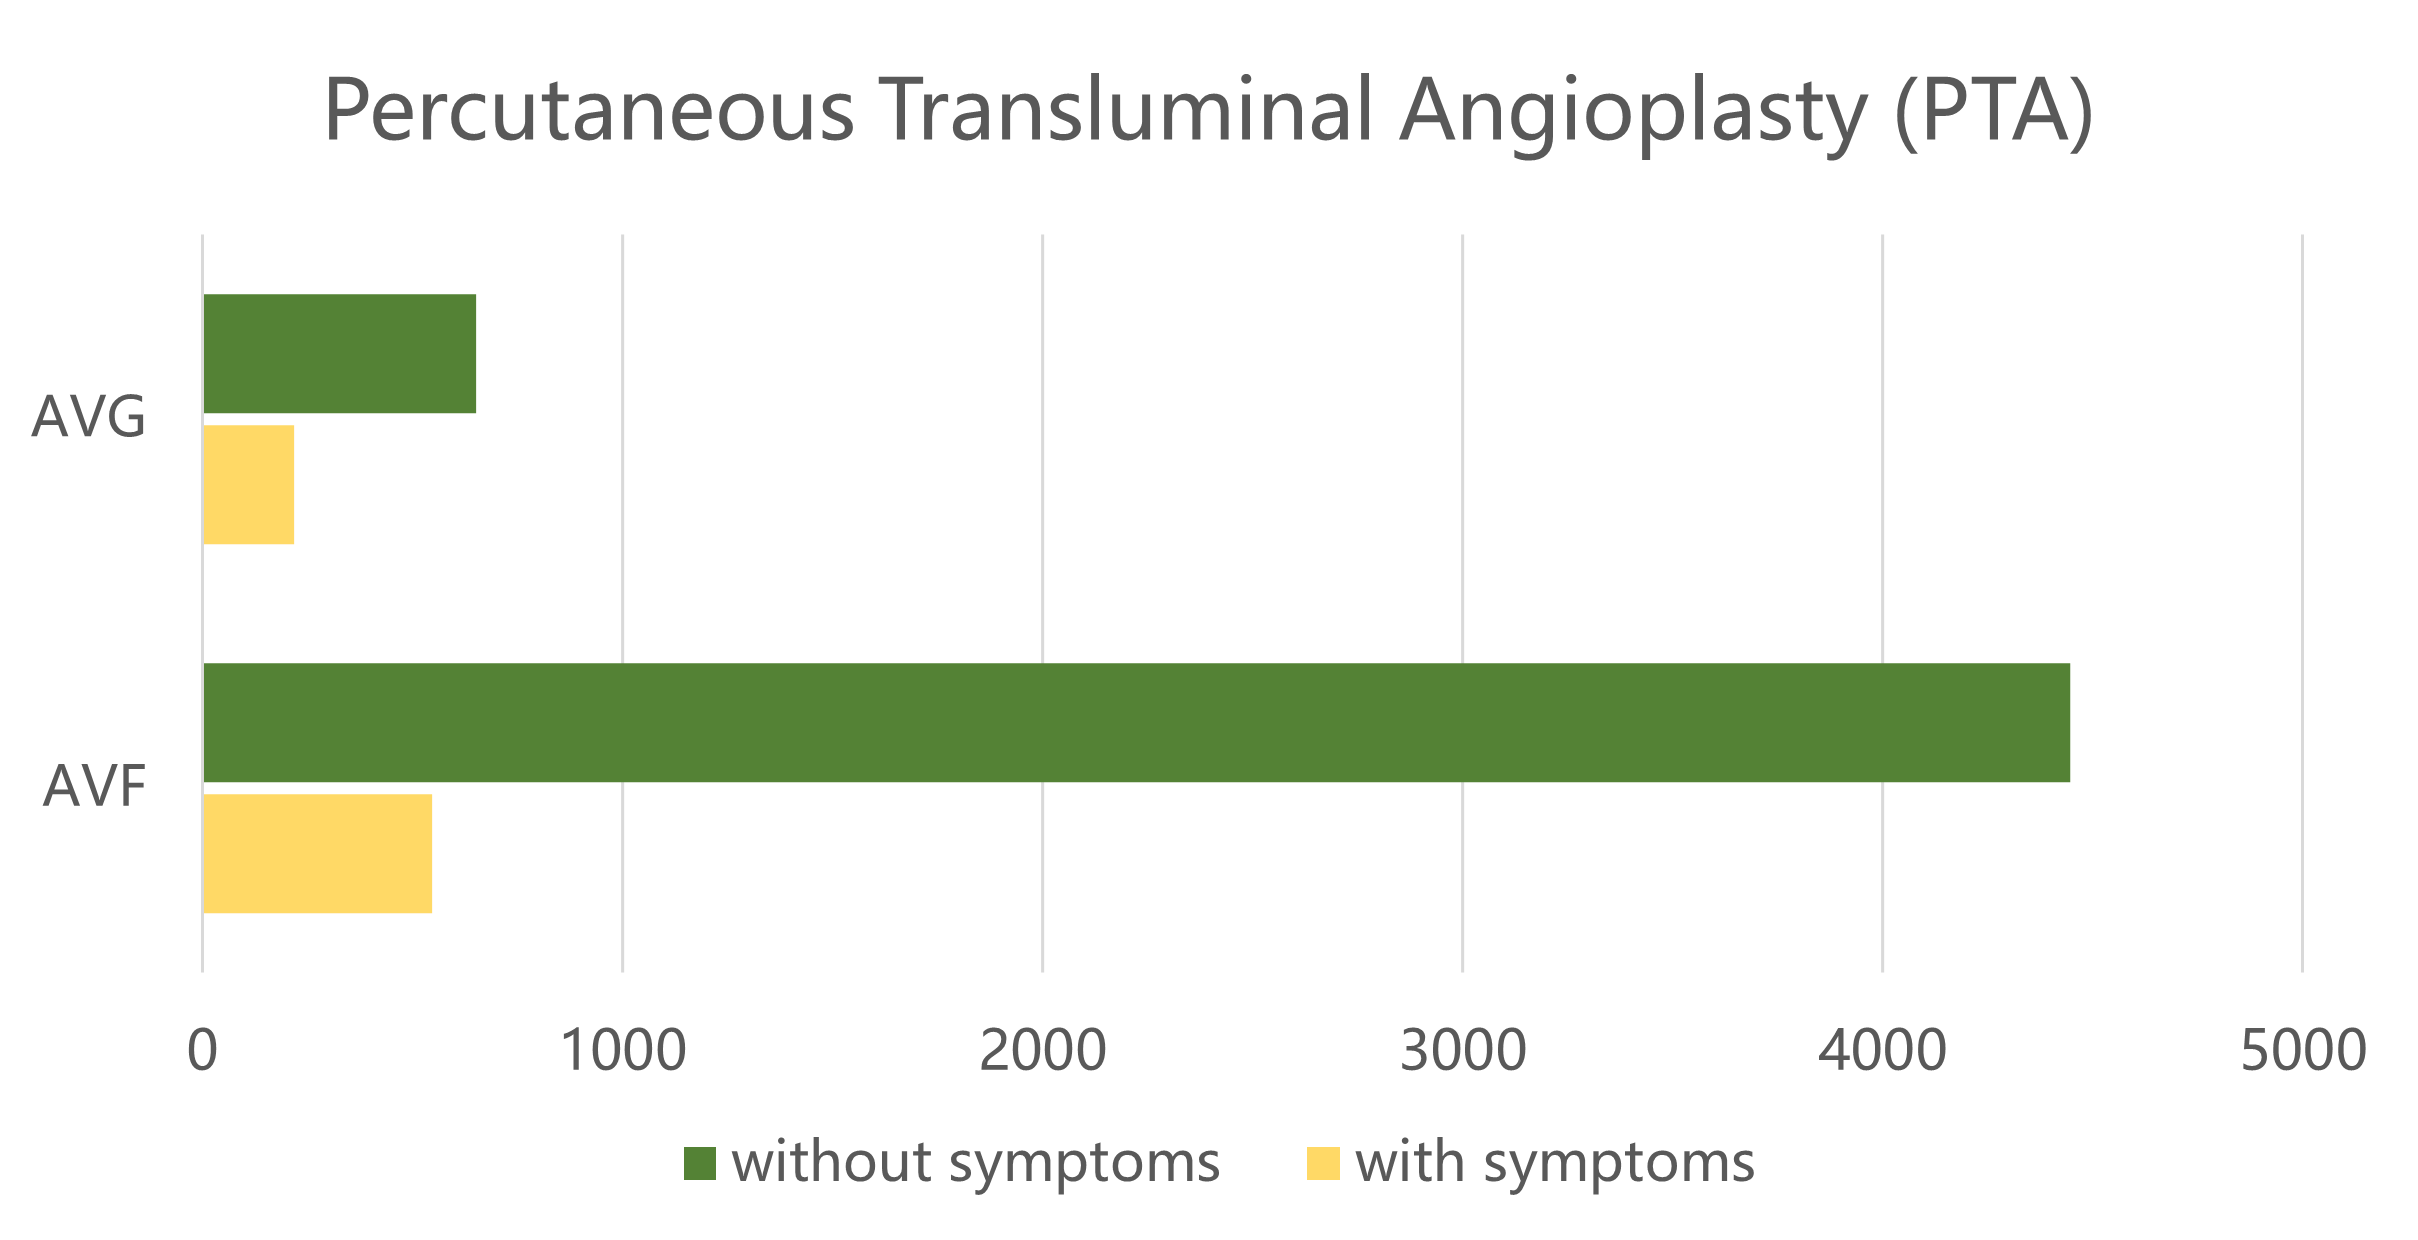
\includegraphics[width=\linewidth]{figures/PTA symptom distribution.png}
        \caption{PTA symptom distribution}
        \label{fig:pta-symptom}
    \end{subfigure}
    \caption{Overview of patient data}
    \label{fig:combined}
\end{figure}

Figure 4.1(a) illustrates the distribution of the dataset based on the type of vascular access. Among the 5,860 records, 85.1\% (4,991 records) belong to patients with AVF, while 14.9\% (869 records) are from patients with AVG. This highlights a significant predominance of AVF cases in the dataset, with AVF records outnumbering AVG records by approximately 6 times. Figure 4.1(b) shows the distribution of patients who underwent PTA procedures, further divided into those with and without symptoms. For AVF patients, the majority did not undergo surgery, with 4,445 (89.1\%) cases categorized as "no PTA," while 546 (10.9\%) cases underwent PTA. Among those who underwent PTA, the majority were asymptomatic. For AVG patients, 651 (74.9\%) cases did not undergo PTA, while 218 (25.1\%) cases underwent PTA. Similar to AVF, most AVG patients who underwent PTA procedures were asymptomatic. However, the proportion of AVG patients undergoing PTA (25.1\%) is significantly higher compared to AVF (10.9\%). The data highlights the disparity in procedural intervention rates between the two vascular access types. AVF patients appear less likely to undergo PTA compared to AVG patients. 

These visualizations emphasize the diversity of patient profiles in the dataset and provide a foundation for the analysis and modeling performed in subsequent sections.
\newpage
\section{Feature Engineering}

To ensure the dataset is suitable for analysis and accurately represents the clinical scenarios, two feature engineering methods were applied: Data Alignment and Feature Creation. These steps enhance the model's ability to capture meaningful patterns and improve prediction performance.

\subsection{Data Alignment}

In the original dataset, there is no Qa value recorded for the day of surgery. Instead, the dataset provides the difference in days between the current record and the previous one. To address this, the record immediately preceding the surgery was selected to represent the surgical day. This approach aligns the data temporally, ensuring that the features used in the model correspond to the patient's most recent clinical status before the procedure. Figure 4.2(b) illustrates the data alignment process.

\begin{figure}[H]
    \centering
    \begin{subfigure}[b]{0.5\textwidth}
        \centering
        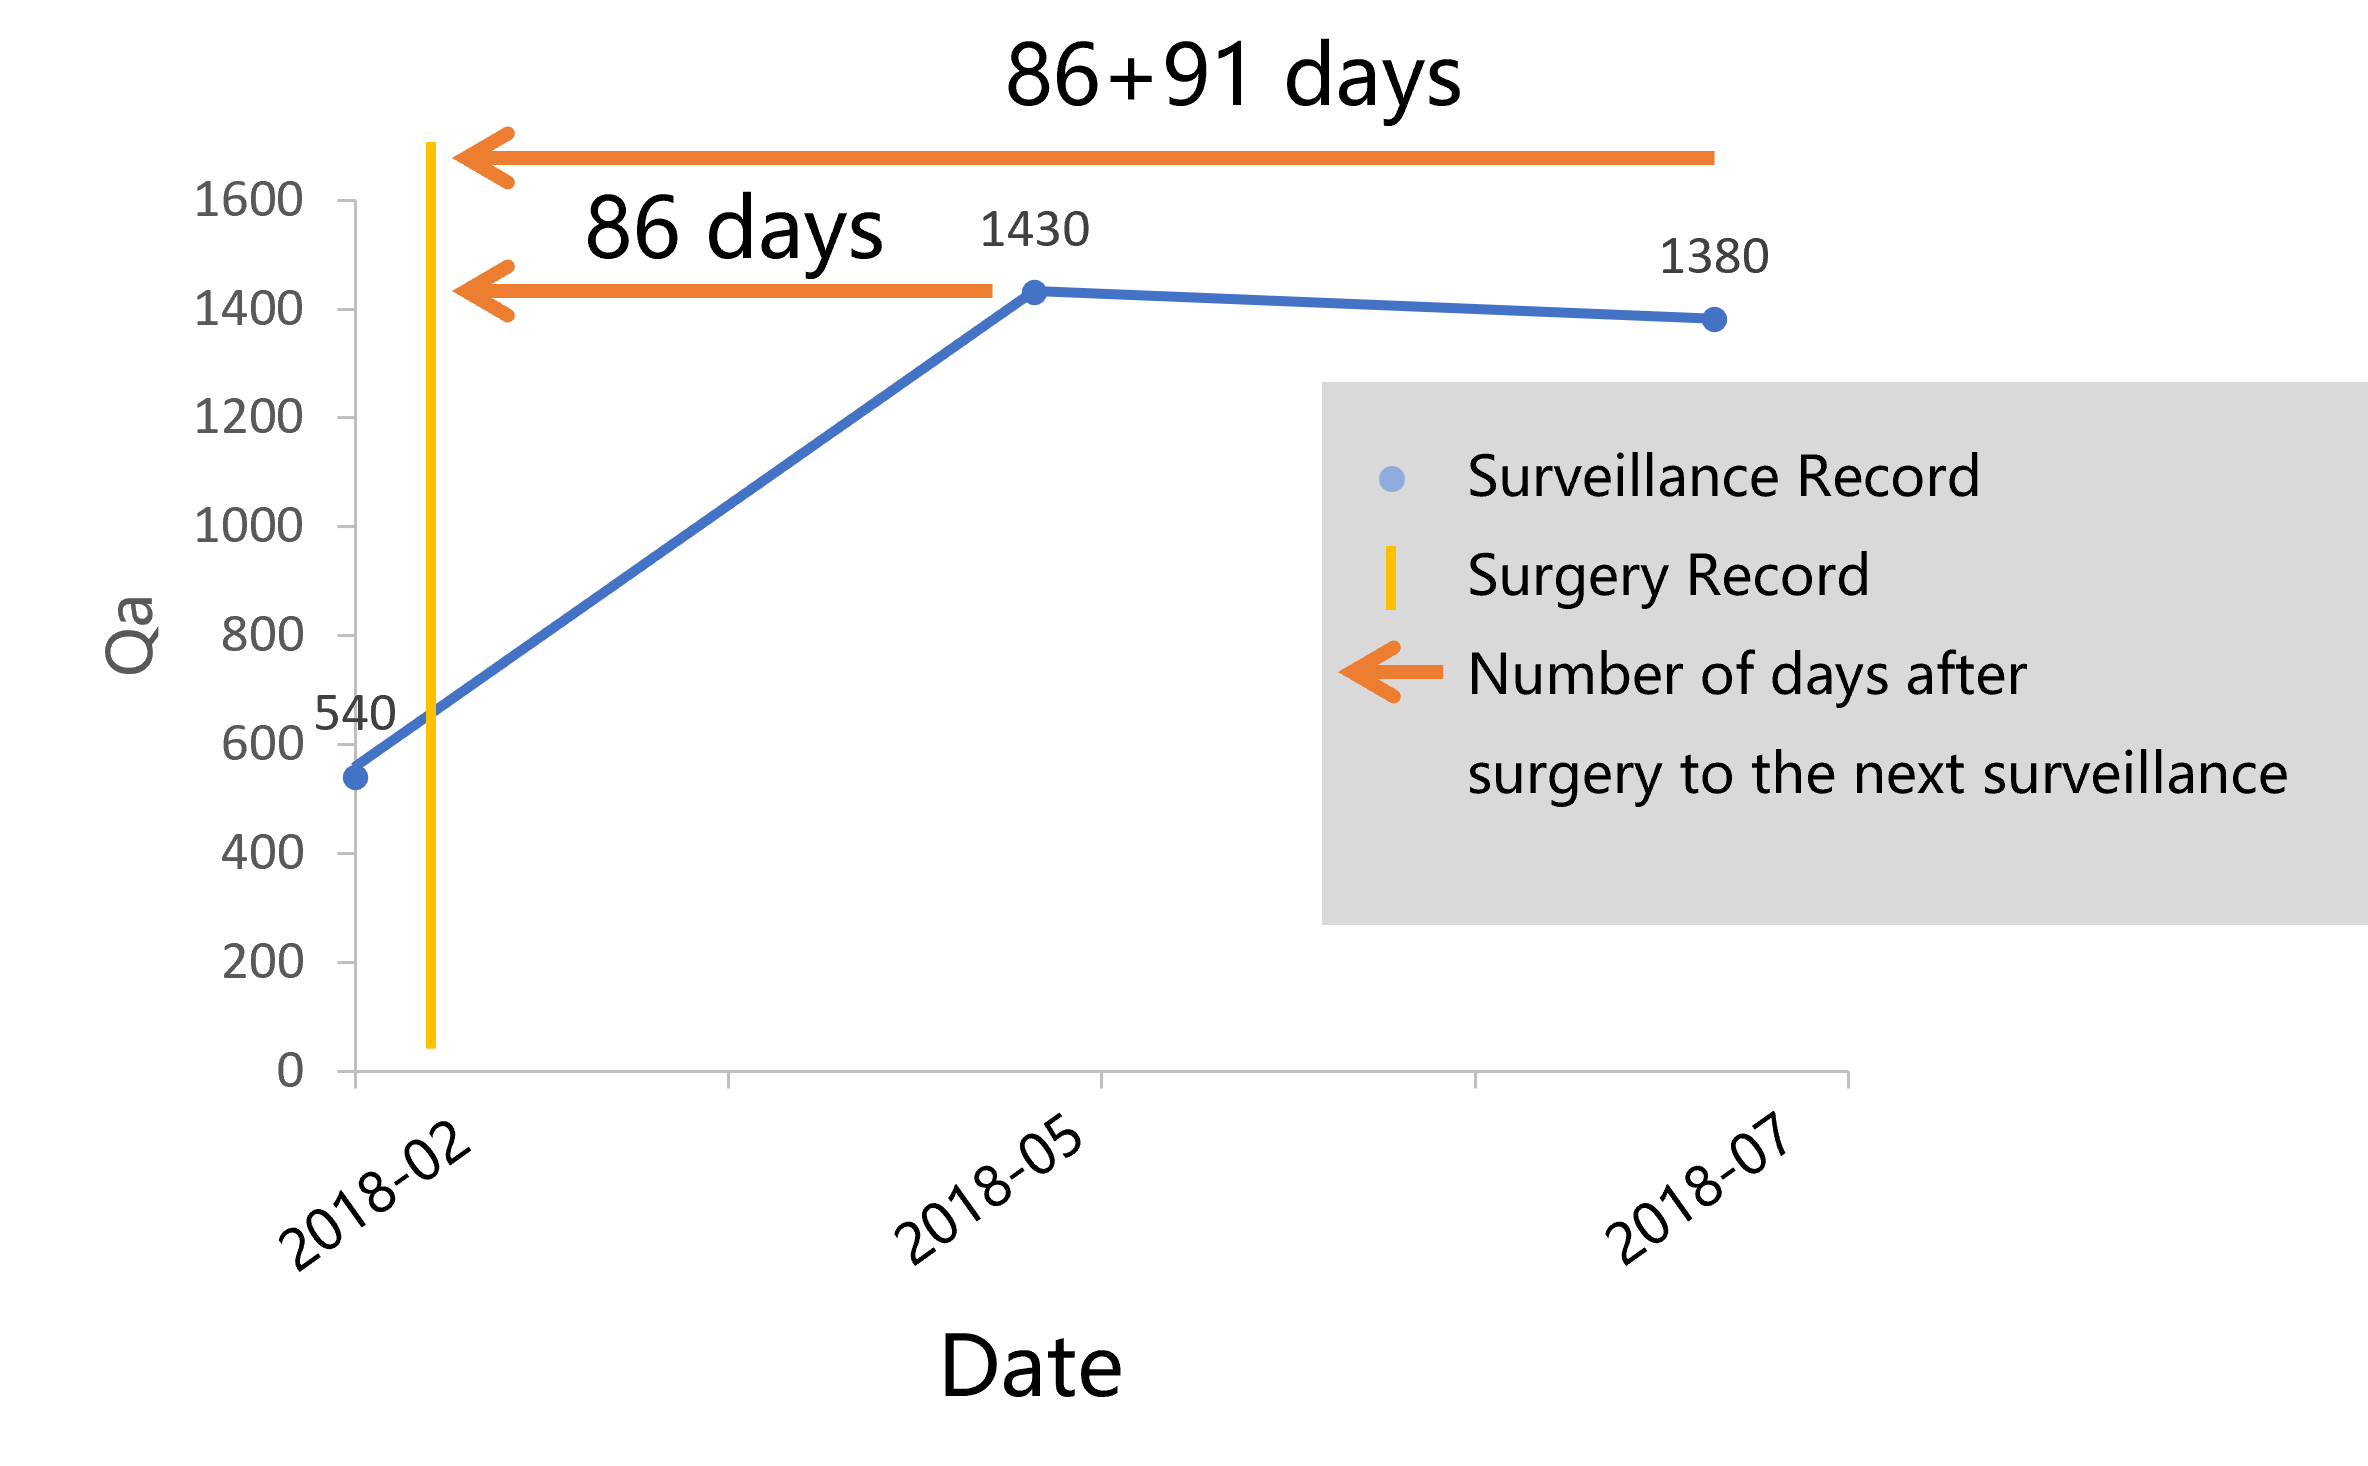
\includegraphics[width=\linewidth]{figures/Patient surveillance and surgery records.png}
        \caption{Patient surveillance and surgery records}
        \label{fig:vascular-access}
    \end{subfigure}%
    \hfill
    \begin{subfigure}[b]{0.4\textwidth}
        \centering
        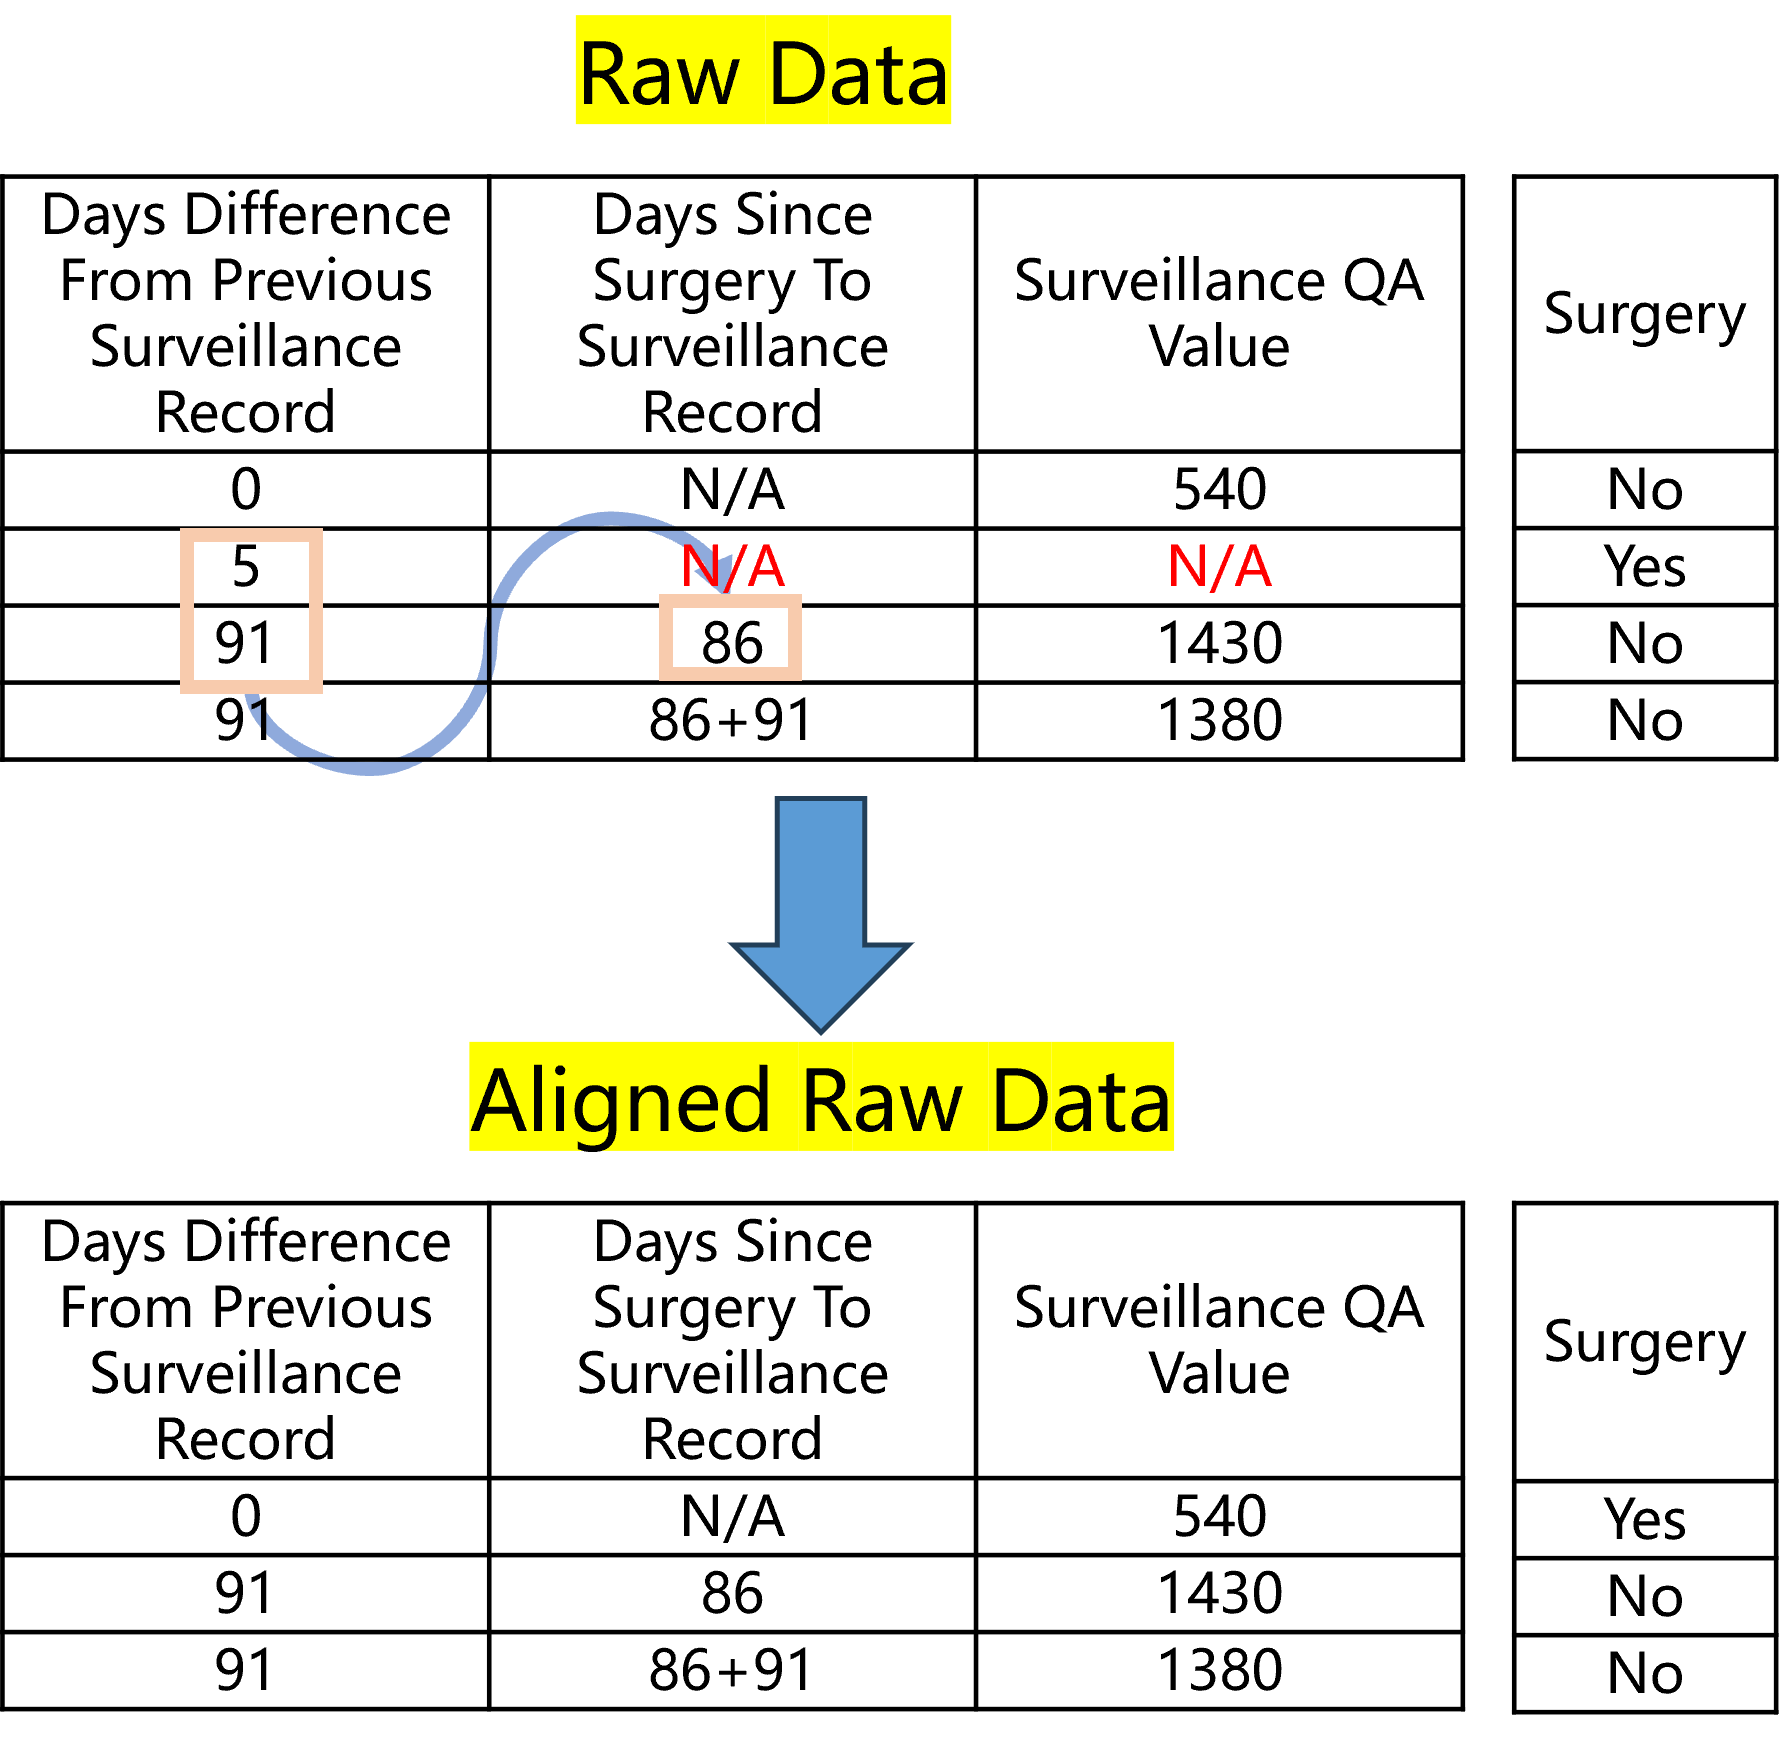
\includegraphics[width=\linewidth]{figures/Data Alignment.png}
        \caption{Data Alignment}
        \label{fig:pta-symptom}
    \end{subfigure}
    \caption{Data alignment process}
    \label{fig:combined}
\end{figure}

\subsection{Feature Creation}

As shown in Figure 4.3, the KDOQI (Kidney Disease Outcomes Quality Initiative) guidelines define three critical features related to vascular access dysfunction: (1) arteriovenous fistula (AVF) with a Qa value less than 400mL/min to 500 mL/min, (2) arteriovenous graft (AVG) with a Qa value less than 600 mL/min, and (3) cases where the Qa value is less than 1000 mL/min and has dropped by 25\%. These features serve as clinically significant indicators for evaluating the performance and functionality of vascular access. Inspired by these guidelines, additional features were created to enhance the model's ability to predict surgical outcomes. These newly created features capture variations in blood flow that may indicate vascular access dysfunction, aiming to provide the model with clinically meaningful variables that align with real-world diagnostic practices. 

\begin{figure}[H]
    \centering
    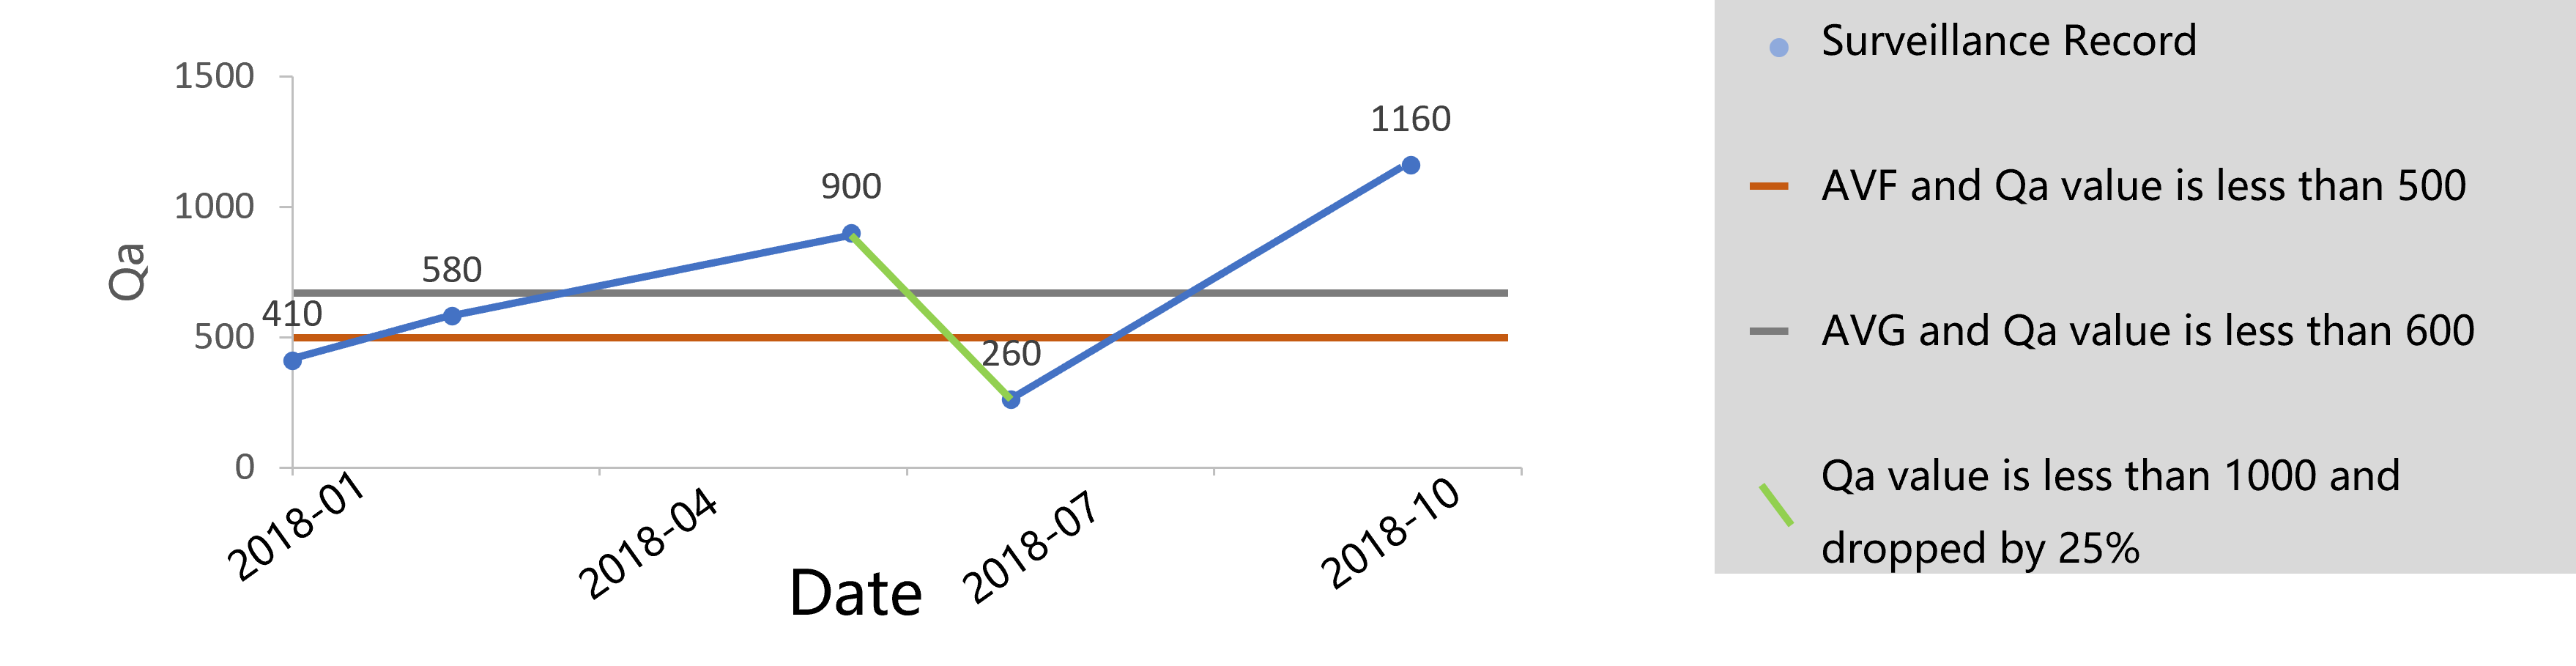
\includegraphics[width=1\linewidth]{figures/KDOQI guidelines.png}
    \caption{KDOQI guidelines feature method to determine whether to perform surgery}
    \label{fig:enter-label}
\end{figure}

To enhance the model's ability to capture historical trends and assess the current state of vascular access functionality, several new features were created. These features provide each sample with information from previous measurements, enabling the model to analyze temporal patterns and changes. The created features are as follows:

\begin{itemize}
    \item \textbf{Qa Value from the Previous Check}: This feature includes the Qa value recorded in the patient's most recent prior check, providing context on the patient's previous vascular access condition.
    \item \textbf{Previous Surgery Indicator}: A binary feature indicating whether a surgical procedure was performed during the previous check. This feature helps identify the impact of recent interventions on the current condition.
    \item \textbf{Slope of Qa Value Difference}: This feature calculates the slope of the Qa value difference between the current and previous measurements, normalized by the number of days elapsed since the last check. It represents the rate of change in Qa value over time, offering a quantitative measure of vascular access deterioration or improvement. The calculation process for this feature is illustrated in Figure 4.4.
    \item \textbf{Difference in Qa Values}: The absolute difference between the current and previous Qa values. This feature captures the magnitude of change in vascular access functionality between two consecutive checks.
\end{itemize}

\begin{figure}[H]
    \centering
    \includegraphics[width=1\linewidth]{figures/The slope of the A value difference between the current and previous measurements relative to the days elapsed since the previous check.png}
    \caption{The slope of the Qa value difference between the current and previous measurements relative to the days elapsed since the previous check}
    \label{fig:enter-label}
\end{figure}

By incorporating these newly created features, each sample is enriched with its historical context, enabling the model to assess trends and variations effectively. The slope and Qa value difference features, in particular, allow the model to detect significant changes in vascular access functionality, which are critical for predicting surgical needs.
\newpage
\section{Evaluation Metrics}

To comprehensively evaluate the performance of the proposed model, we designed an Extended Confusion Matrix that accounts for an additional category of predictions: Indeterminate. This extended framework enables a more nuanced evaluation of model performance, particularly in cases where predictions are inconclusive.

\subsection{Extended Confusion Matrix}

Figure 4.5 shows the Extended Confusion Matrix, which expands upon the traditional confusion matrix by including two new categories:

\begin{itemize}
    \item \textbf{IP (Indeterminate Positive)}: Actual positive cases predicted as indeterminate.
    \item \textbf{IN (Indeterminate Negative)}: Actual negative cases predicted as indeterminate.
\end{itemize}

\begin{figure}[H]
    \centering
    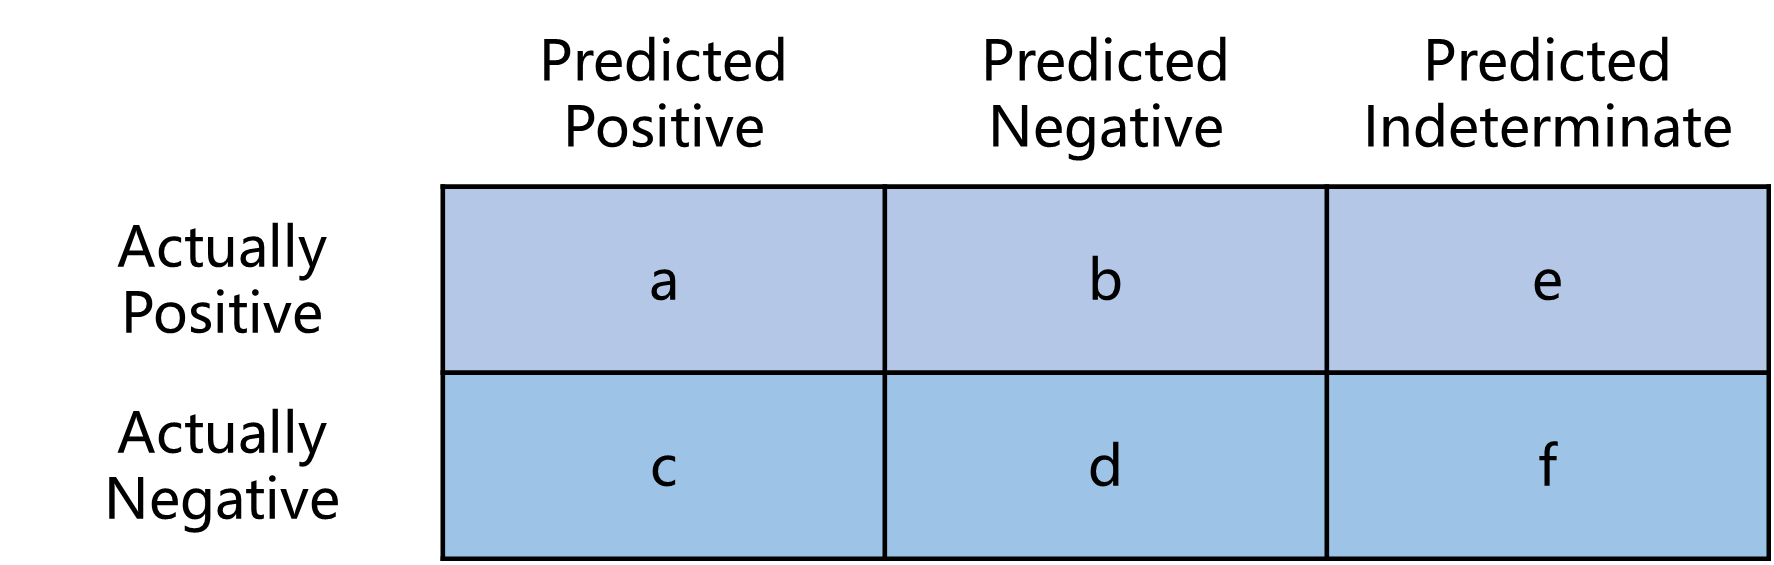
\includegraphics[width=0.6\linewidth]{figures/Extended confusion matrix.png}
    \caption{Extended confusion matrix. a: True Positive (TP), b: False Negative (FN), c: False Positive (FP), d: True Negative (TN), e: Indeterminate Positive (IP), f: Indeterminate Negative (IN)}
    \label{fig:enter-label}
\end{figure}

\subsection{Evaluation Metrics}

Based on Figure 4.5 the Extended Confusion Matrix, we derived several evaluation metrics to measure model performance, including both standard and indeterminacy-aware metrics:

\begin{itemize}
  \item \textbf{Standard Metrics}: 
    \begin{equation}
        Accuracy = \frac{a + d}{a + b + c + d}
    \end{equation}
    \begin{equation}
        PPV = \frac{a}{a + c}
    \end{equation}
    \begin{equation}
        NPV = \frac{d}{b + d}
    \end{equation}
  \item \textbf{Indeterminacy Metrics}: 
    \begin{equation}
        All = a + b + c + d + e + f
    \end{equation}
    \begin{equation}
        Error = \frac{b + c}{All}
    \end{equation}
    \begin{equation}
        Leakage = \frac{b}{All}
    \end{equation}
    \begin{equation}
        Overkill = \frac{c}{All}
    \end{equation}
    \begin{equation}
        Indeterminate = \frac{e + f}{All}
    \end{equation}
    \begin{equation}
        Imperfection = \frac{b + c + e + f}{All}
    \end{equation}
    \begin{equation}
        Indeterminate Recall = \frac{a + e}{a + b + e}
    \end{equation}
    \begin{equation}
        Harmonic\_Score = \frac{\frac{w_1'}{\exp\left(\frac{b}{All}\right)} + \frac{w_2'}{\exp\left(\frac{c}{All}\right)} + \frac{w_3'}{\exp\left(\frac{e + f}{All}\right)}}{3}
    \end{equation}
\end{itemize}

Positive Predictive Value (PPV) evaluates the proportion of predicted positive cases that are actually positive, emphasizing the model’s ability to minimize unnecessary interventions. Negative Predictive Value (NPV) measures the proportion of predicted negative cases that are truly negative, reducing the risk of missed diagnoses. Error Rate quantifies the proportion of all incorrect predictions, providing an overall misclassification rate. Beyond these standard metrics, Leakage Rate captures the proportion of actual positive cases classified as negative, highlighting the risk of failing to detect cases needing intervention, while Overkill Rate measures the proportion of actual negative cases classified as positive, addressing the tendency for over-treatment. Indeterminacy Rate reflects the proportion of predictions classified as indeterminate, enabling the model to flag ambiguous cases for further evaluation. Combining these, the Imperfection Rate aggregates the error and indeterminacy rates to assess the total proportion of samples either misclassified or marked as indeterminate. Additionally, Indeterminate Recall extends the traditional recall metric by including indeterminate positive cases, ensuring the model prioritizes identifying all potential positive cases. Finally, the Harmonic Score provides a balanced measure of leakage, overkill, and indeterminacy rates using weighted components, offering an integrated assessment of the model’s ability to minimize errors, reduce unnecessary interventions, and manage indeterminacy effectively. Together, these metrics form a comprehensive framework for evaluating both the predictive performance and reliability of the model.

\section{Experiment Setup}

In this study, we employed an ensemble learning approach by combining Decision Tree, Random Forest, and XGBoost models into a Soft Voting model. The Decision Tree serves as a base model, providing interpretability for feature impact; Random Forest enhances model robustness through the aggregation of predictions from multiple trees; and XGBoost further improves prediction accuracy with its efficient gradient boosting algorithm. The Soft Voting model integrates the predictions from these individual models using a weighted voting mechanism, achieving overall performance improvement and effectively handling the complexity and indeterminacy in the dataset.

All three models in the Soft Voting ensemble were used with default parameters, except for the \texttt{scale\_pos\_weight} parameter in XGBoost, which was set based on the ratio of patients requiring surgery to those not requiring surgery in the dataset. This adjustment was made to address the data imbalance and ensure the model accurately captured the underrepresented class. The experiments were conducted using a K-fold cross-validation approach with three iterations, and the final results were averaged for consistency. All computations and model training were performed on a high-performance NVIDIA Tesla V100 GPU to ensure efficiency.
\newpage

\section{Experiment Results}

This section summarizes the experimental results for the Arteriovenous Fistula (AVF) and Arteriovenous Graft (AVG) datasets under various parameter settings. By comparing the performance of the KDOQI guidelines with the proposed model, including scenarios where the model incorporates and excludes indeterminate classifications, we evaluate the advantages of our approach in improving diagnostic precision and managing indeterminacy. Key insights are derived from the results of the extended confusion matrix, ROC curves, and the evaluation metrics introduced earlier, highlighting the proposed model’s ability to provide robust and clinically meaningful predictions.

Figures 4.6 illustrate the relationship between the indeterminacy rate and the threshold parameter (\(\theta_{\mu}\)) for the AVF and AVG datasets, respectively. As the threshold increases, the proportion of samples classified as indeterminate decreases, reflecting the model's growing confidence in its predictions. For the AVF dataset, the indeterminacy rate drops from 50\% at a threshold of 0.75 to below 10\% at a threshold of 1.00, while the AVG dataset follows a similar trend, starting at 70\% and decreasing to under 10\%. The higher initial indeterminacy rate for the AVG dataset highlights the increased indeterminacy associated with its smaller sample size and higher proportion of surgical cases. These trends underscore the importance of threshold tuning to balance model confidence and sensitivity to indeterminate cases. A lower threshold captures more ambiguous samples, aiding cautious decision-making, while a higher threshold emphasizes definitive classifications, improving specificity. Based on these findings, we selected a threshold of 0.95, ensuring that the indeterminacy rate remains below 10\% for both datasets. This choice achieves a balance between minimizing indeterminate cases and maintaining high prediction confidence, aligning with the clinical need for precise yet cautious decision-making.

\begin{figure}[H]
    \centering
    \begin{subfigure}[b]{0.5\textwidth}
        \centering
        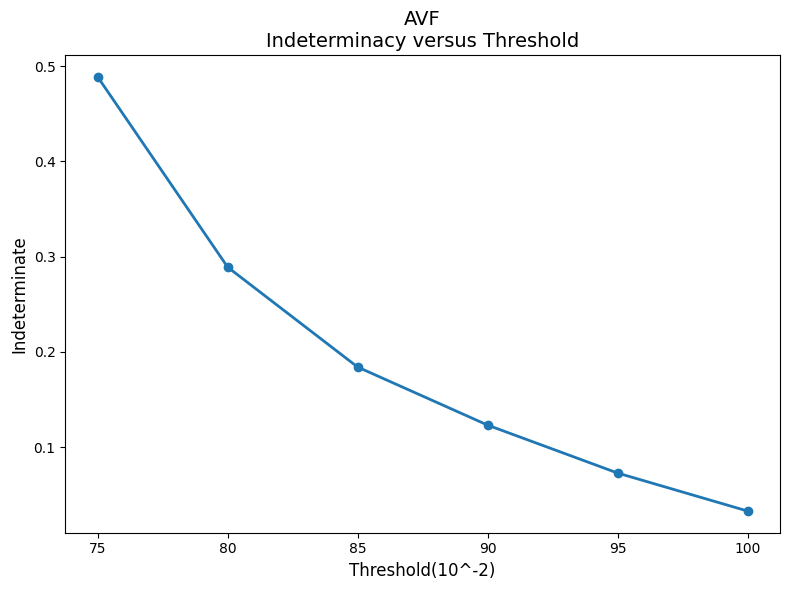
\includegraphics[width=\linewidth]{figures/AVF_Threshold changes used to determine output of indeterminacy.png}
        \caption{Indeterminacy Rate versus Threshold for the AVF Dataset}
        \label{fig:vascular-access}
    \end{subfigure}%
    \hfill
    \begin{subfigure}[b]{0.5\textwidth}
        \centering
        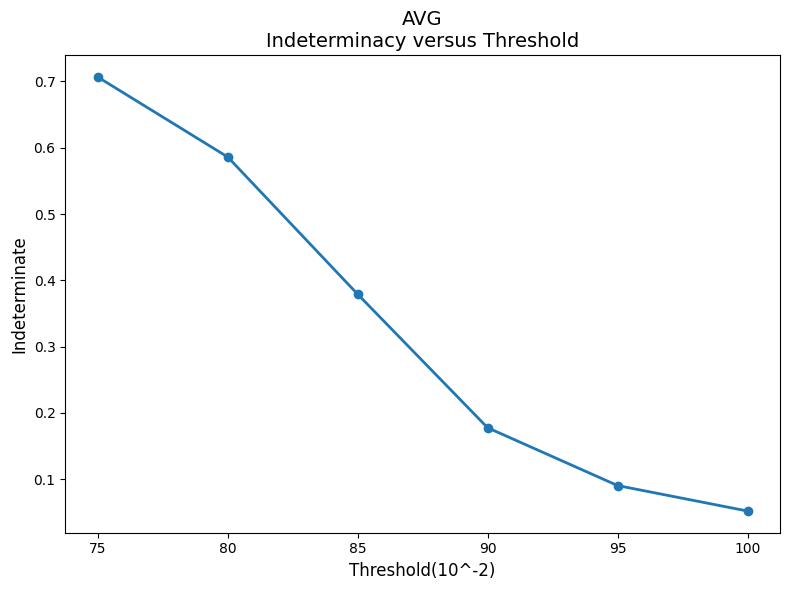
\includegraphics[width=\linewidth]{figures/AVG_Threshold changes used to determine output of indeterminacy.png}
        \caption{Indeterminacy Rate versus Threshold for the AVG Dataset}
        \label{fig:pta-symptom}
    \end{subfigure}
    \caption{Threshold changes used to determine output of indeterminacy}
    \label{fig:combined}
\end{figure}

\subsection{Arteriovenous Fistula Dataset}%AVF

The analysis of the Arteriovenous Fistula (AVF) dataset highlights the significant advantages of the proposed indeterminate-aware model in improving clinical decision-making and addressing indeterminacies in vascular access predictions. This section discusses the experimental results, parameter optimization, and model evaluation, emphasizing the practical implications of the findings.

The parameter settings for the model, determined using Bayesian optimization to maximize accuracy, are presented in Table 4.1. This optimization process identified the best combination of parameters to enhance the model’s predictive performance. 

\begin{table}[H]
    \centering
    \caption{The parameter settings in AVF Dataset}
    \renewcommand{\arraystretch}{1} % 調整行距
    \begin{tabular}[h]{lc} \hline 
        \multicolumn{2}{c}{Parameter Settings} \\ \hline
        Number of estimation times: \(n\) & 10\\ 
        Threshold used to determine output of indeterminacy: \(\theta_{\mu}\) &  0.95\\ 
        Noise mean: \(\mu\) & 0\\ 
        Noise variance: \(\sigma^2\) & 100\\
        Weight of estimator: \(W=[w_{1},w_{2},w_{3}]\) & [1,1,1]\\
        Weight of harmonic score: \(W'=[w_1',w_2',w_3']\) & [1,1,1] \\ \hline 
    \end{tabular}
    \label{tab:Experimental_Config_AVF}
\end{table}

Figure 4.7 illustrates the distribution of the AVF dataset. Out of 4,991 cases, 546 (10.9\%) required PTA interventions, while 4,445 (89.1\%) did not undergo surgery. This imbalance highlights the dataset’s focus on monitoring cases to avoid unnecessary surgical procedures.

\begin{figure}[H]
    \centering
    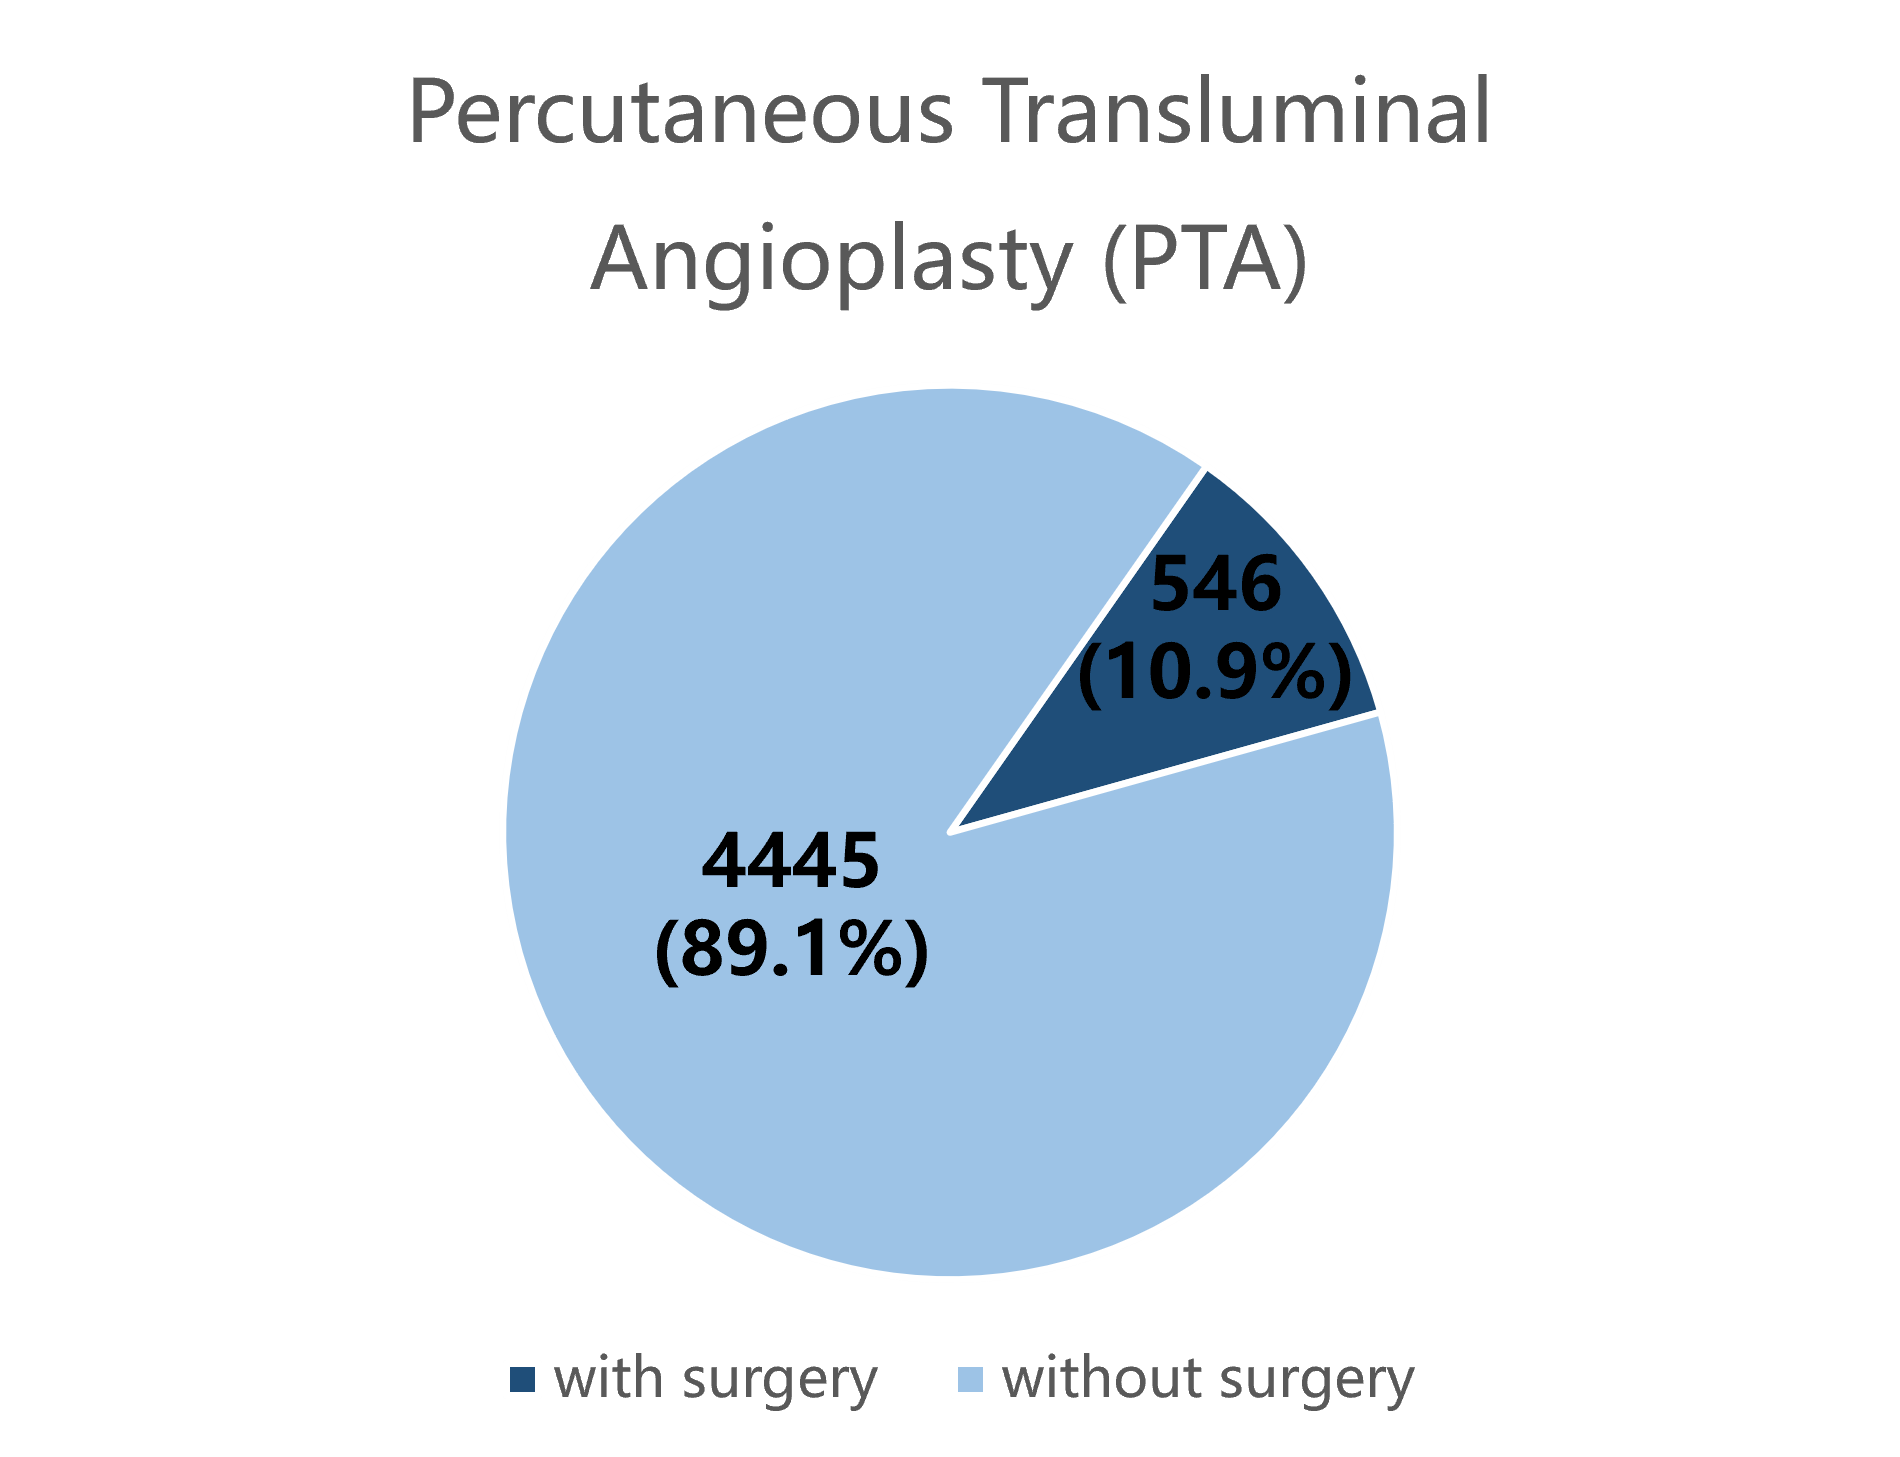
\includegraphics[width=0.7\linewidth]{figures/AVF data distribution.png}
    \caption{AVF data distribution}
    \label{fig:enter-label}
\end{figure}

The comparison of evaluation metrics is detailed in Table 4.2, 4.3, and 4.4, showing results for the KDOQI guidelines, our proposed model without indeterminate classification, and our model with indeterminate classification:

\begin{table}[h]
\centering
% [] 顯示在 list of tables 的文字
% {} 顯示在表格上方的文字
\caption[AVF Dataset Standard Metrics of Baseline, Our Method(Without indeterminate), Our Method(indeterminate)]{AVF Dataset Standard Metrics of Baseline, Our Method(Without indeterminate), Our Method(indeterminate)}
\label{Standard Metrics AVF}
\begin{tabular}{ccccc}
\toprule[1.1pt]
                      & Accuracy & PPV & NPV \\
\midrule[1.1pt]
\multirow{1}{*}{Baseline} & 0.872 ± 0.001 &0.394 ± 0.011 & 0.918 ± 0.003 & \\
\midrule
\multirow{1}{*}{Our Method(Without indeterminate)} & 0.895 ± 0.004 & 0.589 ± 0.028 & 0.904 ± 0.002 \\
\midrule
\multirow{1}{*}{Our Method(indeterminate)} & \textbf{0.913 ± 0.001} & \textbf{0.841 ± 0.043} & 0.914 ± 0.001 \\

\bottomrule[1.1pt]
\end{tabular}
\end{table}


\begin{table}[h]
\centering
% [] 顯示在 list of tables 的文字
% {} 顯示在表格上方的文字
\caption[AVF Dataset Indeterminacy Metrics (I) of Baseline, Our Method(Without indeterminate), Our Method(indeterminate)]{AVF Dataset Indeterminacy Metrics (I) of Baseline, Our Method(Without indeterminate), Our Method(indeterminate)}
\label{Indeterminacy Metrics(I) AVF}
\begin{tabular}{ccccc}
\toprule[1.1pt]
                      & Error & Leakage & Overkill & Indeterminate \\
\midrule[1.1pt]
\multirow{1}{*}{Baseline} & 0.129 ± 0.01 & 0.078 ± 0.012 & 0.051 ± 0.031 & - \\
\midrule
\multirow{1}{*}{Our Method(Without indeterminate)} & 0.105 ± 0.004 & 0.093 ± 0.001 & 0.011 ± 0.003 & - \\
\midrule
\multirow{1}{*}{Our Method(indeterminate)} & \textbf{0.081 ± 0.002} & \textbf{0.08 ± 0.002} & \textbf{0.002 ± 0.002} & 0.073 ± 0.027 \\

\bottomrule[1.1pt]
\end{tabular}
\end{table}

\begin{table}[H]
\centering
% [] 顯示在 list of tables 的文字
% {} 顯示在表格上方的文字
\caption[AVF Dataset Indeterminacy Metrics (II) of Baseline, Our Method(Without indeterminate), Our Method(indeterminate)]{AVF Dataset Indeterminacy Metrics (II) of Baseline, Our Method(Without indeterminate), Our Method(indeterminate)}
\label{Indeterminacy Metrics(II) AVF}
\begin{tabular}{ccccc}
\toprule[1.1pt]
                      & Imperfection & Indeterminate recall & Harmonic score \\
\midrule[1.1pt]
\multirow{1}{*}{Baseline} & 0.129 ± 0.01 & 0.261 ± 0.039 & 0.958 ± 0.002\\
\midrule
\multirow{1}{*}{Our Method(Without indeterminate)} & 0.105 ± 0.004 & 0.146 ± 0.014 & 0.967 ± 0.001 \\
\midrule
\multirow{1}{*}{Our Method(indeterminate)} & 0.154 ± 0.021 & \textbf{0.292 ± 0.03} & 0.951 ± 0.008 \\

\bottomrule[1.1pt]
\end{tabular}
\end{table}

The extended confusion matrix, as shown in Figure 4.8, provides deeper insights into how the model handles ambiguous cases. Unlike the KDOQI guidelines, which classify all cases as either positive or negative, the indeterminate-aware model assigns indeterminate cases to a separate "Indeterminate" category. This approach prevents overly confident misclassifications, particularly for borderline cases where the probability distributions lack clear separation. By reallocating indeterminate predictions, the model reduces the likelihood of errors, ensuring a more cautious and clinically meaningful decision-making process.

\begin{figure}[H]
    \centering
    \begin{subfigure}[b]{0.5\textwidth}
        \centering
        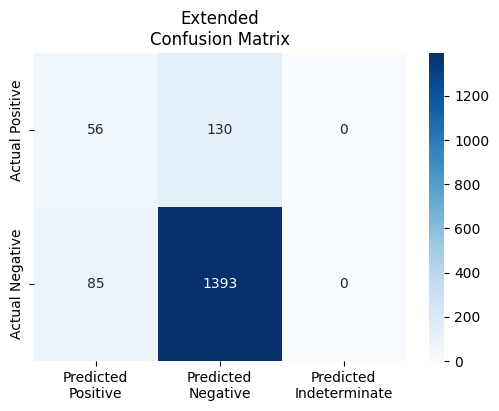
\includegraphics[width=\linewidth]{figures/kdoqi_AVF.png}
        \caption{baseline}
        \label{fig:vascular-access}
    \end{subfigure}
    
    \vspace{1em} % 增加垂直空間

    \begin{subfigure}[b]{0.5\textwidth}
        \centering
        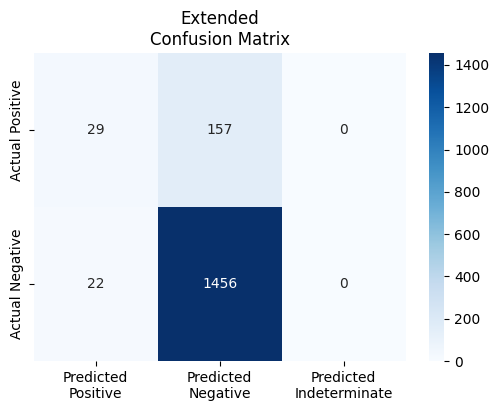
\includegraphics[width=\linewidth]{figures/without_AVF.png}
        \caption{Our Method (Without indeterminate)}
        \label{fig:pta-symptom-method1}
    \end{subfigure}%
    \hfill
    \begin{subfigure}[b]{0.5\textwidth}
        \centering
        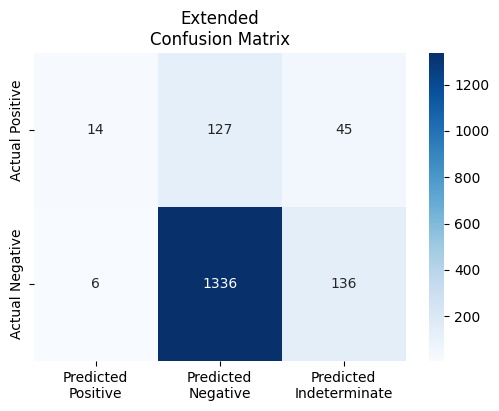
\includegraphics[width=\linewidth]{figures/with_AVF.png}
        \caption{Our Method (Indeterminate)}
        \label{fig:pta-symptom-method2}
    \end{subfigure}

    \caption{AVF Dataset Extended Confusion Matrix}
    \label{fig:combined}
\end{figure}


The ROC curve comparisons, as presented in Figure 4.9, further validate the proposed model's superior discriminative ability. The baseline KDOQI guidelines achieved an AUC of 0.62, reflecting its limited predictive capability. In contrast, the proposed model without indeterminate classification improved to an AUC of 0.73, and the inclusion of indeterminate classifications further enhanced the AUC to 0.76. This progression demonstrates that the model's ability to distinguish between positive and negative cases improves significantly when indeterminacy is explicitly accounted for.

\begin{figure}[H]
    \centering
    \begin{subfigure}[b]{0.5\textwidth}
        \centering
        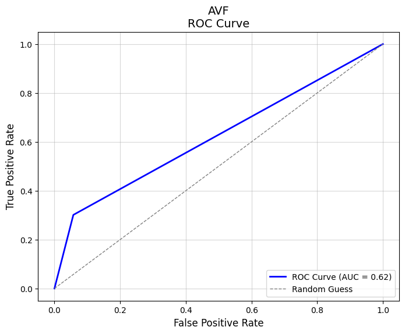
\includegraphics[width=\linewidth]{figures/AVF_baseline_roc.png}
        \caption{baseline}
        \label{fig:vascular-access-roc}
    \end{subfigure}
    
    \vspace{1em} % 增加垂直空間

    \begin{subfigure}[b]{0.5\textwidth}
        \centering
        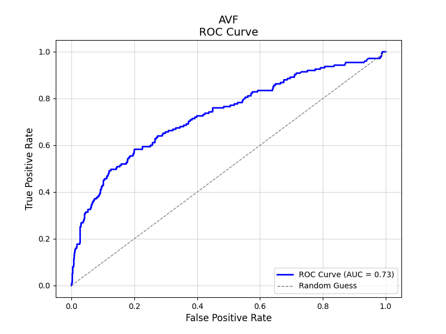
\includegraphics[width=\linewidth]{figures/AVF_method1_roc.png}
        \caption{Our Method (Without indeterminate)}
        \label{fig:pta-symptom-method1-roc}
    \end{subfigure}%
    \hfill
    \begin{subfigure}[b]{0.5\textwidth}
        \centering
        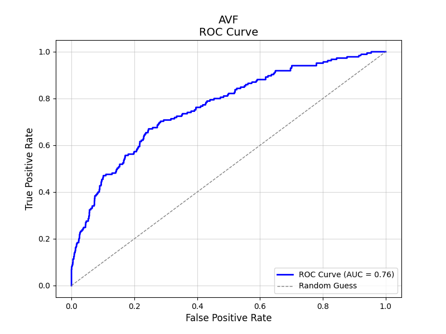
\includegraphics[width=\linewidth]{figures/AVF_method2_roc.png}
        \caption{Our Method (Indeterminate)}
        \label{fig:pta-symptom-method2-roc}
    \end{subfigure}

    \caption{AVF Dataset ROC Curve}
    \label{fig:combined}
\end{figure}

The results from the AVF dataset illustrate the effectiveness of incorporating indeterminate classifications into the prediction framework. The proposed model not only surpasses the KDOQI guidelines in terms of accuracy and precision but also introduces a critical layer of indeterminacy management, which is essential for clinical applications. By balancing standard predictive metrics with indeterminacy-specific measures, the model ensures that ambiguous cases are flagged for further review, reducing the risk of misdiagnoses and unnecessary interventions. These findings underscore the clinical potential of the indeterminate-aware approach for managing vascular access in hemodialysis patients.

\subsection{Arteriovenous Graft Dataset}%AVG

The analysis of the Arteriovenous Graft (AVG) dataset provides complementary insights into the proposed model's performance, particularly in a dataset with fewer samples and a higher proportion of surgical interventions compared to the AVF dataset. This section discusses the dataset characteristics, model evaluation, and the implications of the results.

As shown in Table 4.5, the parameters for the AVG dataset were optimized using Bayesian optimization, which maximized accuracy. 

\begin{table}[H]
    \centering
    \caption{The parameter settings in AVG Dataset}
    \renewcommand{\arraystretch}{1} % 調整行距
    \begin{tabular}[h]{lc} \hline 
        \multicolumn{2}{c}{Parameter Settings} \\ \hline
        Number of estimation times: \(n\) & 10\\ 
        Threshold used to determine output of indeterminacy: \(\theta_{\mu}\) &  0.95\\ 
        Noise mean: \(\mu\) & 0\\ 
        Noise variance: \(\sigma^2\) & 80\\
        Weight of estimator: \(W=[w_{1},w_{2},w_{3}]\) & [1,1,1]\\
        Weight of harmonic score: \(W'=[w_1',w_2',w_3']\) & [1,1,1] \\ \hline 
    \end{tabular}
    \label{tab:Experimental_Config_AVG}
\end{table}

The AVG dataset comprises a total of 869 records, significantly fewer than the 4,991 records in the AVF dataset, as shown in Figure 4.10. Among these records, 218 (25.1\%) involve PTA interventions, while 651 (74.9\%) represent non-surgical cases. The higher proportion of surgical cases in AVG compared to AVF (10.9\%) aligns with clinical observations that AVG is often associated with shorter durability and higher complication rates, necessitating more frequent interventions.

\begin{figure}[H]
    \centering
    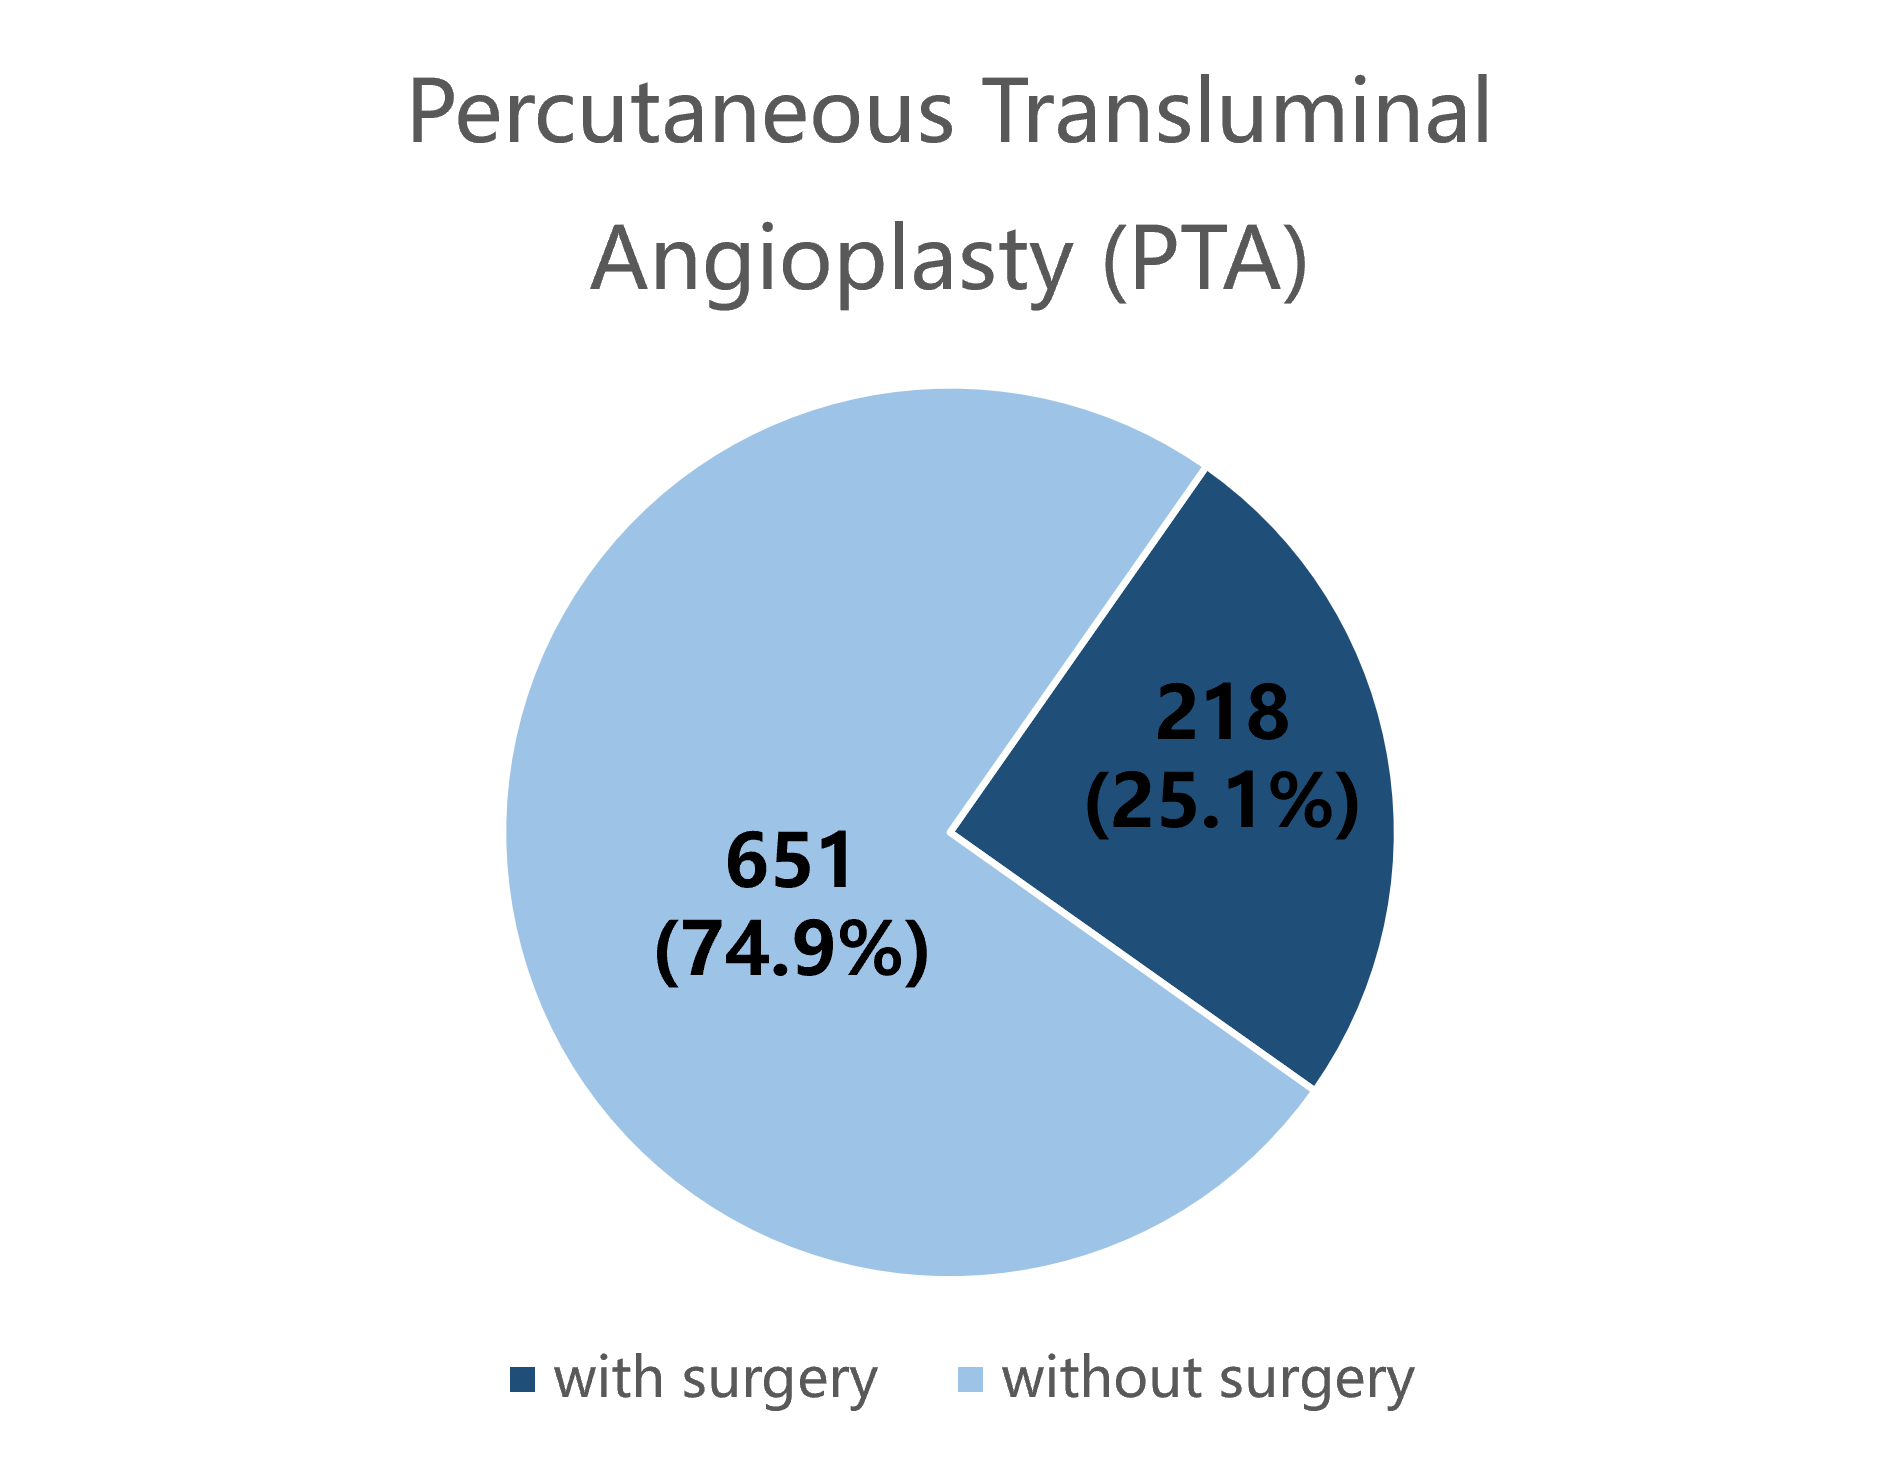
\includegraphics[width=0.7\linewidth]{figures/AVG data distribution.png}
    \caption{AVG data distribution}
    \label{fig:enter-label}
\end{figure}

Tables 4.6, 4.7, and 4.8 show the results of the comparison of metrics between KDOQI guidelines and our method on the AVG dataset.

\begin{table}[h]
\centering
% [] 顯示在 list of tables 的文字
% {} 顯示在表格上方的文字
\caption[AVG Dataset Standard Metrics of Baseline, Our Method(Without indeterminate), Our Method(indeterminate)]{AVG Dataset Standard Metrics of Baseline, Our Method(Without indeterminate), Our Method(indeterminate)}
\label{Standard Metrics AVG}
\begin{tabular}{ccccc}
\toprule[1.1pt]
                      & Accuracy & PPV & NPV \\
\midrule[1.1pt]
\multirow{1}{*}{Baseline} & 0.791 ± 0.018 &0.685 ± 0.044 & 0.809 ± 0.026 & \\
\midrule
\multirow{1}{*}{Our Method(Without indeterminate)} & 0.765 ± 0.023 & 0.695 ± 0.045 & 0.788 ± 0.028 \\
\midrule
\multirow{1}{*}{Our Method(indeterminate)} & \textbf{0.818 ± 0.019} & \textbf{0.74 ± 0.137} & \textbf{0.828 ± 0.031} \\

\bottomrule[1.1pt]
\end{tabular}
\end{table}


\begin{table}[h]
\centering
% [] 顯示在 list of tables 的文字
% {} 顯示在表格上方的文字
\caption[AVG Dataset Indeterminacy Metrics (I) of Baseline, Our Method(Without indeterminate), Our Method(indeterminate)]{AVG Dataset Indeterminacy Metrics (I) of Baseline, Our Method(Without indeterminate), Our Method(indeterminate)}
\label{Indeterminacy Metrics(I) AVG}
\begin{tabular}{ccccc}
\toprule[1.1pt]
                      & Error & Leakage & Overkill & Indeterminate \\
\midrule[1.1pt]
\multirow{1}{*}{Baseline} & 0.208 ± 0.032 & 0.186 ± 0.011 & 0.048 ± 0.016 & - \\
\midrule
\multirow{1}{*}{Our Method(Without indeterminate)} & 0.235 ± 0.023 & 0.19 ± 0.027 & 0.032 ± 0.017 & - \\
\midrule
\multirow{1}{*}{Our Method(indeterminate)} & \textbf{0.147 ± 0.017} & \textbf{0.128 ± 0.025} & \textbf{0.02 ± 0.011} & 0.192 ± 0.007 \\

\bottomrule[1.1pt]
\end{tabular}
\end{table}

\begin{table}[H]
\centering
% [] 顯示在 list of tables 的文字
% {} 顯示在表格上方的文字
\caption[AVG Dataset Indeterminacy Metrics (II) of Baseline, Our Method(Without indeterminate), Our Method(indeterminate)]{AVG Dataset Indeterminacy Metrics (II) of Baseline, Our Method(Without indeterminate), Our Method(indeterminate)}
\label{Indeterminacy Metrics(II) AVG}
\begin{tabular}{ccccc}
\toprule[1.1pt]
                      & Imperfection & Indeterminate recall & Harmonic score \\
\midrule[1.1pt]
\multirow{1}{*}{Baseline} & 0.208 ± 0.032 & 0.262 ± 0.07 & 0.908 ± 0.018\\
\midrule
\multirow{1}{*}{Our Method(Without indeterminate)} & 0.235 ± 0.023 & 0.247 ± 0.059 & 0.928 ± 0.013 \\
\midrule
\multirow{1}{*}{Our Method(indeterminate)} & 0.34 ± 0.011 & \textbf{0.496 ± 0.059} & 0.895 ± 0.013 \\

\bottomrule[1.1pt]
\end{tabular}
\end{table}

The extended confusion matrix in Figure 4.11 shows how the proposed model reallocates a significant proportion of indeterminate predictions to the "Indeterminate" category. Compared to AVF, the higher surgical proportion in AVG is evident in the relative distribution of predicted positive and negative cases. The indeterminate-aware approach ensures that borderline cases are cautiously flagged, avoiding overconfidence in predictions.

\begin{figure}[H]
    \centering
    \begin{subfigure}[b]{0.5\textwidth}
        \centering
        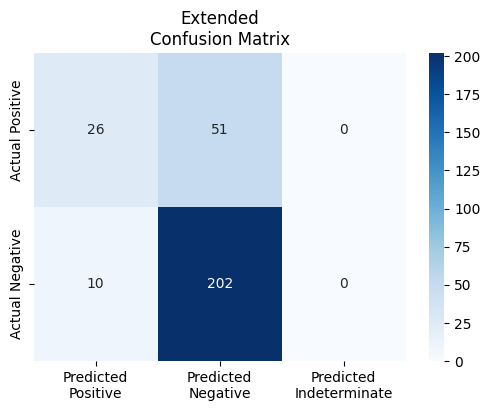
\includegraphics[width=\linewidth]{figures/kdoqi_AVG.png}
        \caption{baseline}
        \label{fig:vascular-access}
    \end{subfigure}
    
    \vspace{1em} % 增加垂直空間

    \begin{subfigure}[b]{0.5\textwidth}
        \centering
        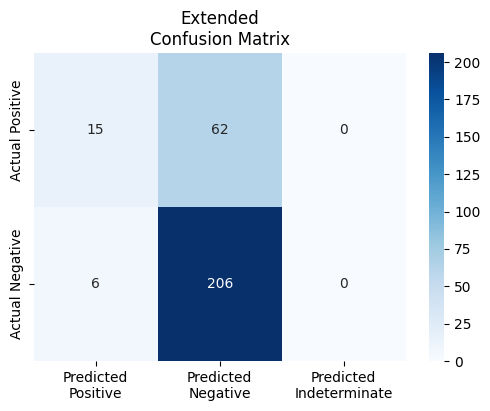
\includegraphics[width=\linewidth]{figures/without_AVG.png}
        \caption{Our Method (Without indeterminate)}
        \label{fig:pta-symptom-method1}
    \end{subfigure}%
    \hfill
    \begin{subfigure}[b]{0.5\textwidth}
        \centering
        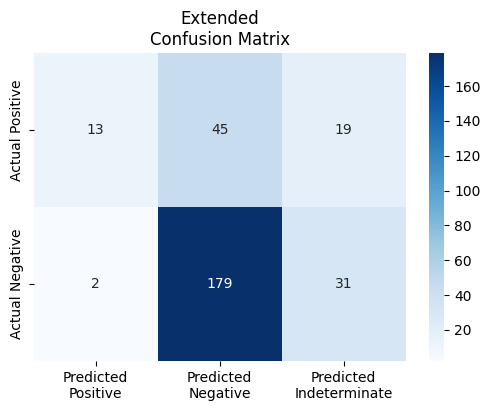
\includegraphics[width=\linewidth]{figures/with_AVG.png}
        \caption{Our Method (Indeterminate)}
        \label{fig:pta-symptom-method2}
    \end{subfigure}

    \caption{AVG Dataset Extended Confusion Matrix}
    \label{fig:combined}
\end{figure}

The ROC curve analysis, illustrated in Figure 4.12, shows the progression of AUC values across configurations. The baseline KDOQI guidelines achieved an AUC of 0.62, reflecting its limited predictive capability. The proposed model without indeterminate classification achieved an AUC of 0.64, while the inclusion of indeterminate classifications further improved the AUC to 0.73. These results demonstrate that explicitly accounting for indeterminacy enhances the model’s ability to distinguish between positive and negative cases.

\begin{figure}[H]
    \centering
    \begin{subfigure}[b]{0.5\textwidth}
        \centering
        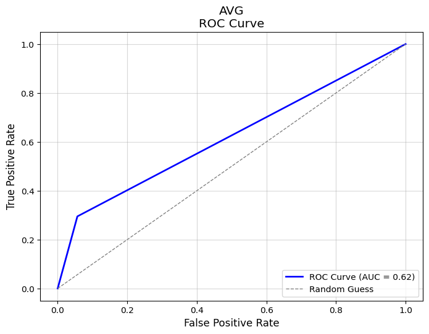
\includegraphics[width=\linewidth]{figures/AVG_baseline_roc.png}
        \caption{baseline}
        \label{fig:vascular-access-roc}
    \end{subfigure}
    
    \vspace{1em} % 增加垂直空間

    \begin{subfigure}[b]{0.5\textwidth}
        \centering
        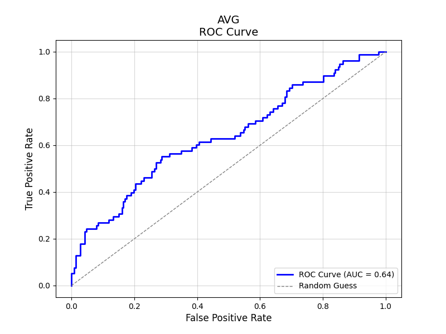
\includegraphics[width=\linewidth]{figures/AVG_method1_roc.png}
        \caption{Our Method (Without indeterminate)}
        \label{fig:pta-symptom-method1-roc}
    \end{subfigure}%
    \hfill
    \begin{subfigure}[b]{0.5\textwidth}
        \centering
        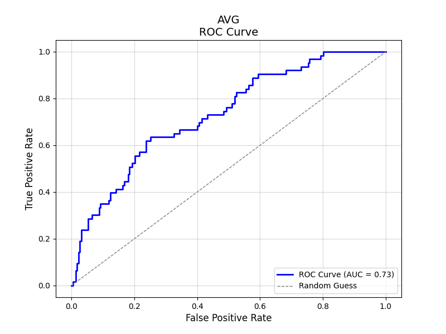
\includegraphics[width=\linewidth]{figures/AVG_method2_roc.png}
        \caption{Our Method (Indeterminate)}
        \label{fig:pta-symptom-method2-roc}
    \end{subfigure}

    \caption{AVG Dataset ROC Curve}
    \label{fig:combined}
\end{figure}

In comparison to the AVF dataset, the AVG dataset presents unique challenges due to its smaller size and higher surgical intervention rate. Despite these differences, the proposed indeterminate-aware model consistently outperformed both the KDOQI guidelines and the model without indeterminate classifications. The results emphasize the model’s adaptability and robustness, making it a valuable tool for supporting clinical decision-making in vascular access management.
\chapter{Conclusion}
In this paper, we proposed an innovative concept of a compositional conditional diffusion model to generate unseen defect component. We in a method based on class-image correlation to regulate the diffusion model for image generation. The outcomes of this research can be applied in the context of defect detection in electronic industry production lines. When encountering new defective components in the future, the compositional conditional diffusion model can be employed to generate visual representations of these components. The produced images can then be incorporated into the defect detection model for further training.

This research project aims to investigate the practical aspects of human composite cognitive abilities, emphasizing the process of learning from existing composite concepts and applying them to novel composite concepts. Specifically, in the domain of image generation, the goal is to achieve "composite zero-shot image generation and selection." Within the academic realm of artificial intelligence, the study delves into the generalization capabilities of neural networks in the context of composite zero-shot learning and generation. We look forward to further exploring the compositional condition diffusion model in a wider variety of settings and data modalities.
\label{chapter:fig}


%-------------------------------------------------------------------------------
% 參考文獻
%-------------------------------------------------------------------------------

% Set bib style
\bibliographystyle{IEEEtran}


% Add Bibliography to "Table of Contents"
\addBibToContents

% Usage:
%   \bibliography{bib/bib1,bib/bib2,...,bib/bibN} % 注意: 不要有空格
%
% For IEEEtran users:
%   DO NOT remove bib/BSTcontrol.bib when using IEEEtran.bst. The reason is that
% when we cite two papers of the same (or similar) authors, IEEEtran.bst would
% replace the author names with "------". To avoid this, we use BSTControl.bib
% to set ctldash_repeated_names to 'no'.
%
% For non IEEEtran users:
%   Please delete bib/ieeeBSTcontrol from \bibliography{}
\bibliography{bib/ieeeBSTcontrol,bib/thesis}

%-------------------------------------------------------------------------------
% 附錄
%-------------------------------------------------------------------------------

% Start appendix
\appendix

% Add appendicies to "Table of Contents"
\addAppxToContents

% 請從此開始依序擺放附錄
%\chapter{附錄標題}

%\section{Testing}


%-------------------------------------------------------------------------------
% 作者簡歷
%-------------------------------------------------------------------------------

% 簡歷 (Only shown in a PhD dissertation)
\begin{vita}%

{\bf Harry Potter} is a character in TJ. K. Rowling's magic wonderland, ``Harry Potter." His research interests are finding the ways to trigger the catastrophe in Hogwarts.

\end{vita}

% 著作列表 (Only shown in a PhD dissertation)
\begin{publications}%

%%%%%%%%%%%%%%%%%%%%%%%%%%%%%%%%%%%%%%%%%%%%%%%%%%%%%%%%%%%%%%%%%%%%%%%%%%%%%%%

\section*{Journal Papers}
\begin{spacing}{1}
\begin{enumerate}

\item {\bf \underline{Harry Potter}}, Albus Dumbledore, ``The way to beat the dark lord, from Love to Horcrux," \textit{Journal of Supplementary}, vol. 777, no. 1, pp. 11--21, 2021

\end{enumerate}
\end{spacing}

%%%%%%%%%%%%%%%%%%%%%%%%%%%%%%%%%%%%%%%%%%%%%%%%%%%%%%%%%%%%%%%%%%%%%%%%%%%%%%%

\section*{Conference Papers}
\begin{spacing}{1}
\begin{enumerate}

\item {\bf \underline{害你駁倒}}, ``校園毀滅計畫," in \textit{International Conference of School Refresh}, 2021, Hogwarts, England

\end{enumerate}
\end{spacing}

%%%%%%%%%%%%%%%%%%%%%%%%%%%%%%%%%%%%%%%%%%%%%%%%%%%%%%%%%%%%%%%%%%%%%%%%%%%%%%%

\end{publications}

\end{document}